% Options for packages loaded elsewhere
\PassOptionsToPackage{unicode}{hyperref}
\PassOptionsToPackage{hyphens}{url}
%
\documentclass[
]{article}
\title{Internet News and Consumer Engagement}
\author{Muhammad Daaboul}
\date{17 October 2021}

\usepackage{amsmath,amssymb}
\usepackage{lmodern}
\usepackage{iftex}
\ifPDFTeX
  \usepackage[T1]{fontenc}
  \usepackage[utf8]{inputenc}
  \usepackage{textcomp} % provide euro and other symbols
\else % if luatex or xetex
  \usepackage{unicode-math}
  \defaultfontfeatures{Scale=MatchLowercase}
  \defaultfontfeatures[\rmfamily]{Ligatures=TeX,Scale=1}
\fi
% Use upquote if available, for straight quotes in verbatim environments
\IfFileExists{upquote.sty}{\usepackage{upquote}}{}
\IfFileExists{microtype.sty}{% use microtype if available
  \usepackage[]{microtype}
  \UseMicrotypeSet[protrusion]{basicmath} % disable protrusion for tt fonts
}{}
\makeatletter
\@ifundefined{KOMAClassName}{% if non-KOMA class
  \IfFileExists{parskip.sty}{%
    \usepackage{parskip}
  }{% else
    \setlength{\parindent}{0pt}
    \setlength{\parskip}{6pt plus 2pt minus 1pt}}
}{% if KOMA class
  \KOMAoptions{parskip=half}}
\makeatother
\usepackage{xcolor}
\IfFileExists{xurl.sty}{\usepackage{xurl}}{} % add URL line breaks if available
\IfFileExists{bookmark.sty}{\usepackage{bookmark}}{\usepackage{hyperref}}
\hypersetup{
  pdftitle={Internet News and Consumer Engagement},
  pdfauthor={Muhammad Daaboul},
  hidelinks,
  pdfcreator={LaTeX via pandoc}}
\urlstyle{same} % disable monospaced font for URLs
\usepackage[margin=1in]{geometry}
\usepackage{color}
\usepackage{fancyvrb}
\newcommand{\VerbBar}{|}
\newcommand{\VERB}{\Verb[commandchars=\\\{\}]}
\DefineVerbatimEnvironment{Highlighting}{Verbatim}{commandchars=\\\{\}}
% Add ',fontsize=\small' for more characters per line
\usepackage{framed}
\definecolor{shadecolor}{RGB}{248,248,248}
\newenvironment{Shaded}{\begin{snugshade}}{\end{snugshade}}
\newcommand{\AlertTok}[1]{\textcolor[rgb]{0.94,0.16,0.16}{#1}}
\newcommand{\AnnotationTok}[1]{\textcolor[rgb]{0.56,0.35,0.01}{\textbf{\textit{#1}}}}
\newcommand{\AttributeTok}[1]{\textcolor[rgb]{0.77,0.63,0.00}{#1}}
\newcommand{\BaseNTok}[1]{\textcolor[rgb]{0.00,0.00,0.81}{#1}}
\newcommand{\BuiltInTok}[1]{#1}
\newcommand{\CharTok}[1]{\textcolor[rgb]{0.31,0.60,0.02}{#1}}
\newcommand{\CommentTok}[1]{\textcolor[rgb]{0.56,0.35,0.01}{\textit{#1}}}
\newcommand{\CommentVarTok}[1]{\textcolor[rgb]{0.56,0.35,0.01}{\textbf{\textit{#1}}}}
\newcommand{\ConstantTok}[1]{\textcolor[rgb]{0.00,0.00,0.00}{#1}}
\newcommand{\ControlFlowTok}[1]{\textcolor[rgb]{0.13,0.29,0.53}{\textbf{#1}}}
\newcommand{\DataTypeTok}[1]{\textcolor[rgb]{0.13,0.29,0.53}{#1}}
\newcommand{\DecValTok}[1]{\textcolor[rgb]{0.00,0.00,0.81}{#1}}
\newcommand{\DocumentationTok}[1]{\textcolor[rgb]{0.56,0.35,0.01}{\textbf{\textit{#1}}}}
\newcommand{\ErrorTok}[1]{\textcolor[rgb]{0.64,0.00,0.00}{\textbf{#1}}}
\newcommand{\ExtensionTok}[1]{#1}
\newcommand{\FloatTok}[1]{\textcolor[rgb]{0.00,0.00,0.81}{#1}}
\newcommand{\FunctionTok}[1]{\textcolor[rgb]{0.00,0.00,0.00}{#1}}
\newcommand{\ImportTok}[1]{#1}
\newcommand{\InformationTok}[1]{\textcolor[rgb]{0.56,0.35,0.01}{\textbf{\textit{#1}}}}
\newcommand{\KeywordTok}[1]{\textcolor[rgb]{0.13,0.29,0.53}{\textbf{#1}}}
\newcommand{\NormalTok}[1]{#1}
\newcommand{\OperatorTok}[1]{\textcolor[rgb]{0.81,0.36,0.00}{\textbf{#1}}}
\newcommand{\OtherTok}[1]{\textcolor[rgb]{0.56,0.35,0.01}{#1}}
\newcommand{\PreprocessorTok}[1]{\textcolor[rgb]{0.56,0.35,0.01}{\textit{#1}}}
\newcommand{\RegionMarkerTok}[1]{#1}
\newcommand{\SpecialCharTok}[1]{\textcolor[rgb]{0.00,0.00,0.00}{#1}}
\newcommand{\SpecialStringTok}[1]{\textcolor[rgb]{0.31,0.60,0.02}{#1}}
\newcommand{\StringTok}[1]{\textcolor[rgb]{0.31,0.60,0.02}{#1}}
\newcommand{\VariableTok}[1]{\textcolor[rgb]{0.00,0.00,0.00}{#1}}
\newcommand{\VerbatimStringTok}[1]{\textcolor[rgb]{0.31,0.60,0.02}{#1}}
\newcommand{\WarningTok}[1]{\textcolor[rgb]{0.56,0.35,0.01}{\textbf{\textit{#1}}}}
\usepackage{longtable,booktabs,array}
\usepackage{calc} % for calculating minipage widths
% Correct order of tables after \paragraph or \subparagraph
\usepackage{etoolbox}
\makeatletter
\patchcmd\longtable{\par}{\if@noskipsec\mbox{}\fi\par}{}{}
\makeatother
% Allow footnotes in longtable head/foot
\IfFileExists{footnotehyper.sty}{\usepackage{footnotehyper}}{\usepackage{footnote}}
\makesavenoteenv{longtable}
\usepackage{graphicx}
\makeatletter
\def\maxwidth{\ifdim\Gin@nat@width>\linewidth\linewidth\else\Gin@nat@width\fi}
\def\maxheight{\ifdim\Gin@nat@height>\textheight\textheight\else\Gin@nat@height\fi}
\makeatother
% Scale images if necessary, so that they will not overflow the page
% margins by default, and it is still possible to overwrite the defaults
% using explicit options in \includegraphics[width, height, ...]{}
\setkeys{Gin}{width=\maxwidth,height=\maxheight,keepaspectratio}
% Set default figure placement to htbp
\makeatletter
\def\fps@figure{htbp}
\makeatother
\setlength{\emergencystretch}{3em} % prevent overfull lines
\providecommand{\tightlist}{%
  \setlength{\itemsep}{0pt}\setlength{\parskip}{0pt}}
\setcounter{secnumdepth}{-\maxdimen} % remove section numbering
\ifLuaTeX
  \usepackage{selnolig}  % disable illegal ligatures
\fi

\begin{document}
\maketitle


\includegraphics{banner.png}

Ready to put your coding skills to the test? Join us for our Workspace
Competition.\\
For more information, visit
\href{https://datacamp.com/workspacecompetition}{datacamp.com/workspacecompetition}

\hypertarget{context}{%
\subsubsection{Context}\label{context}}

This dataset
(\href{https://www.kaggle.com/szymonjanowski/internet-articles-data-with-users-engagement}{source})
consists of data about news articles collected from Sept.~3, 2019 until
Nov.~4, 2019. Afterwards, it is enriched by Facebook engagement data,
such as number of shares, comments and reactions. It was first created
to predict the popularity of an article before it was published.
However, there is a lot more you can analyze; take a look at some
suggestions at the end of this template.

\hypertarget{load-packages}{%
\subsubsection{Load packages}\label{load-packages}}

\begin{Shaded}
\begin{Highlighting}[]
\FunctionTok{library}\NormalTok{(skimr)}
\FunctionTok{library}\NormalTok{(tidyverse)}
\end{Highlighting}
\end{Shaded}

\hypertarget{load-your-data}{%
\subsubsection{Load your Data}\label{load-your-data}}

\begin{Shaded}
\begin{Highlighting}[]
\NormalTok{articles }\OtherTok{\textless{}{-}}\NormalTok{ readr}\SpecialCharTok{::}\FunctionTok{read\_csv}\NormalTok{(}\StringTok{\textquotesingle{}data/news\_articles.csv.gz\textquotesingle{}}\NormalTok{)}
\NormalTok{articles}\SpecialCharTok{$}\NormalTok{source\_id }\OtherTok{\textless{}{-}} \FunctionTok{as.factor}\NormalTok{(articles}\SpecialCharTok{$}\NormalTok{source\_id)}
\NormalTok{articles}\SpecialCharTok{$}\NormalTok{source\_name }\OtherTok{\textless{}{-}} \FunctionTok{as.factor}\NormalTok{(articles}\SpecialCharTok{$}\NormalTok{source\_name)}
\FunctionTok{skim}\NormalTok{(articles) }\SpecialCharTok{\%\textgreater{}\%} 
  \FunctionTok{select}\NormalTok{(}\SpecialCharTok{{-}}\NormalTok{(numeric.p0}\SpecialCharTok{:}\NormalTok{numeric.p100)) }\SpecialCharTok{\%\textgreater{}\%}
  \FunctionTok{select}\NormalTok{(}\SpecialCharTok{{-}}\NormalTok{(complete\_rate))}
\end{Highlighting}
\end{Shaded}

\begin{longtable}[]{@{}ll@{}}
\caption{Data summary}\tabularnewline
\toprule
\endhead
Name & articles \\
Number of rows & 10437 \\
Number of columns & 15 \\
\_\_\_\_\_\_\_\_\_\_\_\_\_\_\_\_\_\_\_\_\_\_\_ & \\
Column type frequency: & \\
character & 6 \\
factor & 2 \\
numeric & 6 \\
POSIXct & 1 \\
\_\_\_\_\_\_\_\_\_\_\_\_\_\_\_\_\_\_\_\_\_\_\_\_ & \\
Group variables & None \\
\bottomrule
\end{longtable}

\textbf{Variable type: character}

\begin{longtable}[]{@{}lrrrrrr@{}}
\toprule
skim\_variable & n\_missing & min & max & empty & n\_unique &
whitespace \\
\midrule
\endhead
author & 1020 & 2 & 184 & 0 & 2580 & 0 \\
title & 2 & 5 & 250 & 0 & 9810 & 0 \\
description & 24 & 3 & 266 & 0 & 9173 & 0 \\
url & 1 & 34 & 325 & 0 & 10433 & 0 \\
url\_to\_image & 656 & 31 & 261 & 0 & 8363 & 0 \\
content & 1292 & 26 & 276 & 0 & 8385 & 0 \\
\bottomrule
\end{longtable}

\textbf{Variable type: factor}

\begin{longtable}[]{@{}lrlrl@{}}
\toprule
skim\_variable & n\_missing & ordered & n\_unique & top\_counts \\
\midrule
\endhead
source\_id & 0 & FALSE & 13 & reu: 1252, bbc: 1242, the: 1232, abc:
1139 \\
source\_name & 0 & FALSE & 13 & Reu: 1252, BBC: 1242, The: 1232, ABC:
1139 \\
\bottomrule
\end{longtable}

\textbf{Variable type: numeric}

\begin{longtable}[]{@{}lrrrl@{}}
\toprule
skim\_variable & n\_missing & mean & sd & hist \\
\midrule
\endhead
\ldots1 & 0 & 5218.00 & 3013.05 & ▇▇▇▇▇ \\
top\_article & 2 & 0.12 & 0.33 & ▇▁▁▁▁ \\
engagement\_reaction\_count & 118 & 381.40 & 4433.34 & ▇▁▁▁▁ \\
engagement\_comment\_count & 118 & 124.03 & 965.35 & ▇▁▁▁▁ \\
engagement\_share\_count & 118 & 196.24 & 1020.68 & ▇▁▁▁▁ \\
engagement\_comment\_plugin\_count & 118 & 0.01 & 0.27 & ▇▁▁▁▁ \\
\bottomrule
\end{longtable}

\textbf{Variable type: POSIXct}

\begin{longtable}[]{@{}lrlllr@{}}
\toprule
skim\_variable & n\_missing & min & max & median & n\_unique \\
\midrule
\endhead
published\_at & 1 & 2019-09-03 & 2019-10-03 17:49:31 & 2019-09-12
18:32:38 & 9439 \\
\bottomrule
\end{longtable}

\hypertarget{understand-your-data}{%
\subsubsection{Understand your data}\label{understand-your-data}}

\begin{longtable}[]{@{}
  >{\raggedright\arraybackslash}p{(\columnwidth - 2\tabcolsep) * \real{0.30}}
  >{\raggedright\arraybackslash}p{(\columnwidth - 2\tabcolsep) * \real{0.70}}@{}}
\toprule
\begin{minipage}[b]{\linewidth}\raggedright
Variable.
\end{minipage} & \begin{minipage}[b]{\linewidth}\raggedright
Description
\end{minipage} \\
\midrule
\endhead
source\_id & publisher unique identifier \\
source\_name & human-readable publisher name \\
author & article author \\
title & article headline \\
description & article short description \\
url & article URL from publisher website \\
url\_to\_image & URL to main image associated with the article \\
published\_at & exact time and date of publishing the article \\
content & unformatted content of the article truncated to 260
characters \\
top\_article & value indicating if article was listed as a top article
on publisher website \\
engagement\_reaction\_count & users reactions count for posts on
Facebook involving article URL \\
engagement\_comment\_count & users comments count for posts on Facebook
involving article URL \\
engagement\_share\_count & users shares count for posts on Facebook
involving article URL \\
engagement\_comment\_plugin\_count & Users comments count for Facebook
comment plugin on article website \\
\bottomrule
\end{longtable}

Now you can start to explore this dataset with the chance to win
incredible prices! Can't think of where to start? Try your hand at these
suggestions:

\begin{itemize}
\tightlist
\item
  Extract useful insights and visualize them in the most interesting way
  possible.
\item
  Categorize the articles into different categories based on, for
  example, sentiment.
\item
  Cluster the news articles, authors or publishers based on, for
  example, topic.
\item
  Make a title generator based on data such as content, description,
  etc.
\end{itemize}

\hypertarget{judging-criteria}{%
\subsubsection{Judging Criteria}\label{judging-criteria}}

\begin{longtable}[]{@{}lll@{}}
\toprule
CATEGORY & WEIGHTAGE & DETAILS \\
\midrule
\endhead
\textbf{Analysis} & 30\% & \\
\textbf{Results} & 30\% & \\
\textbf{Creativity} & 40\% & \\
\bottomrule
\end{longtable}

\hypertarget{understanding-our-dataset}{%
\subsection{Understanding our dataset}\label{understanding-our-dataset}}

We observe that the \texttt{articles} dataset has 10,436 articles that
have been published by 12 of the biggest names in the news industry. Our
objective is to gain a deeper understanding of the relationship between
these different news providers with particular emphasis on Reuters. We
intend to cover the following four main areas in our analysis:

\begin{itemize}
\tightlist
\item
  Topic correlation
\item
  Sentiment analysis
\item
  Topic modeling for cluster analysis\\
\item
  Understand the main triggers behind popularity
\end{itemize}

We present below an extract from the first row of this dataset to help
build the readers intuition of the main elements that will be effective
in our analysis.

\textbf{Source}: 10

\textbf{Author}: Reuters Editorial

\textbf{Published at}: 1567527740

\textbf{URL TO IMAGE}:

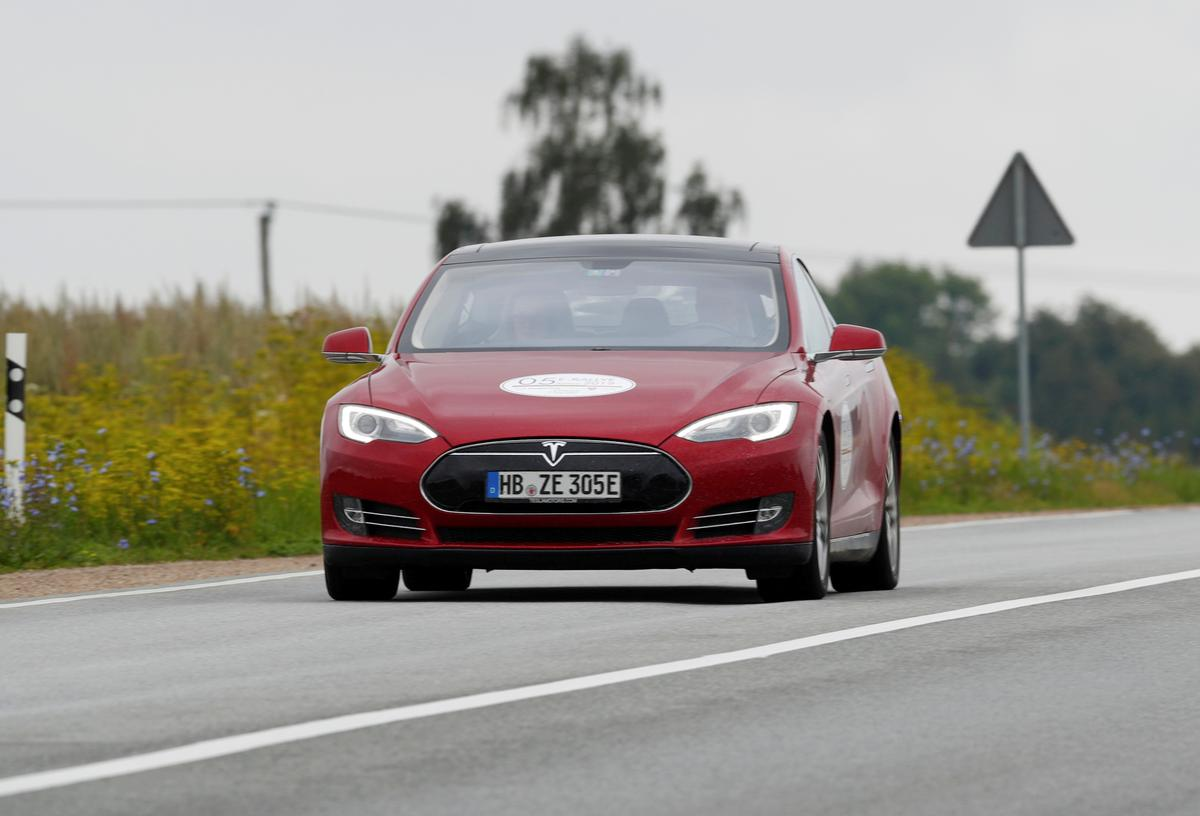
\includegraphics{car.png}

\textbf{Title}: NTSB says Autopilot engaged in 2018 California Tesla
crash

\textbf{Description}: The National Transportation Safety Board said
Tuesday a Tesla Model S was in Autopilot mode when it struck a fire
truck in Culver City, California -- one of a series of crashes the board
is investigating involving Tesla's driver assistance system.

\textbf{Content}: WASHINGTON (Reuters) - The National Transportation
Safety Board said Tuesday a Tesla Model S was in Autopilot mode when it
struck a fire truck in Culver City, California one of a series of
crashes the board is investigating involving Tesla's driver
assistance\ldots{} {[}+478 chars{]}

\textbf{Reaction}: 0 times


\includegraphics{facebook-reactions.png}

\textbf{Comments}: 0 times

\textbf{Shares}: 2528 times

This article however was not recorded to have had any reactions or
comments, but was shared 2528 times ! Other information that would also
be included but not found for article under id no. 1 would be:

\begin{itemize}
\tightlist
\item
  engagement\_reaction\_count
\item
  engagement\_comment\_count
\item
  engagement\_comment\_plugin\_count
\end{itemize}

Now that we have a feel of how the contents we can also view these using
the \texttt{str()} function as shown below to view the first article's
content:

\begin{Shaded}
\begin{Highlighting}[]
\FunctionTok{str}\NormalTok{(articles[}\DecValTok{1}\NormalTok{,])}
\end{Highlighting}
\end{Shaded}

\begin{verbatim}
## tibble [1 x 15] (S3: tbl_df/tbl/data.frame)
##  $ ...1                           : num 0
##  $ source_id                      : Factor w/ 13 levels "1","abc-news",..: 10
##  $ source_name                    : Factor w/ 13 levels "460.0","ABC News",..: 10
##  $ author                         : chr "Reuters Editorial"
##  $ title                          : chr "NTSB says Autopilot engaged in 2018 California Tesla crash"
##  $ description                    : chr "The National Transportation Safety Board said Tuesday a Tesla Model S was in Autopilot mode when it struck a fi"| __truncated__
##  $ url                            : chr "https://www.reuters.com/article/us-tesla-crash-idUSKCN1VO22E"
##  $ url_to_image                   : chr "https://s4.reutersmedia.net/resources/r/?m=02&d=20190903&t=2&i=1425817142&w=1200&r=LYNXNPEF821HS"
##  $ published_at                   : POSIXct[1:1], format: "2019-09-03 16:22:20"
##  $ content                        : chr "WASHINGTON (Reuters) - The National Transportation Safety Board said Tuesday a Tesla Model S was in Autopilot m"| __truncated__
##  $ top_article                    : num 0
##  $ engagement_reaction_count      : num 0
##  $ engagement_comment_count       : num 0
##  $ engagement_share_count         : num 2528
##  $ engagement_comment_plugin_count: num 0
\end{verbatim}

We will also use the \texttt{source\_name} column going forward rather
than the \texttt{source\_id} column. We have verified below that there
are no differences between these two columns, but have chosen the former
simply because it looks a lot neater and is more suitable for use for
our graphical representations going forward.

\begin{Shaded}
\begin{Highlighting}[]
\NormalTok{articles }\SpecialCharTok{\%\textgreater{}\%}
  \FunctionTok{count}\NormalTok{(source\_id, source\_name)}
\end{Highlighting}
\end{Shaded}

\begin{verbatim}
## # A tibble: 13 x 3
##    source_id               source_name                 n
##    <fct>                   <fct>                   <int>
##  1 1                       460.0                       1
##  2 abc-news                ABC News                 1139
##  3 al-jazeera-english      Al Jazeera English        499
##  4 bbc-news                BBC News                 1242
##  5 business-insider        Business Insider         1048
##  6 cbs-news                CBS News                  952
##  7 cnn                     CNN                      1132
##  8 espn                    ESPN                       82
##  9 newsweek                Newsweek                  539
## 10 reuters                 Reuters                  1252
## 11 the-irish-times         The Irish Times          1232
## 12 the-new-york-times      The New York Times        986
## 13 the-wall-street-journal The Wall Street Journal   333
\end{verbatim}

We start by summarizing key the main article engagement metrics
gathered. It would be misleading to compare the total number of
reactions, comments, or shares irrespective of the number of articles
related to each news provider. We will therefore present the
\texttt{mean} which will allow us to form a reasonable comparison
between users different behaviours towards the different news source
providers.

\begin{Shaded}
\begin{Highlighting}[]
\NormalTok{articles }\SpecialCharTok{\%\textgreater{}\%}
 \FunctionTok{filter}\NormalTok{(}\SpecialCharTok{!}\NormalTok{source\_name }\SpecialCharTok{==} \StringTok{"460.0"}\NormalTok{) }\SpecialCharTok{\%\textgreater{}\%}
 \FunctionTok{group\_by}\NormalTok{(source\_name) }\SpecialCharTok{\%\textgreater{}\%}
 \FunctionTok{summarise}\NormalTok{(}\AttributeTok{reaction =} \FunctionTok{mean}\NormalTok{(engagement\_reaction\_count),}
            \AttributeTok{comment =} \FunctionTok{mean}\NormalTok{(engagement\_comment\_count),}
              \AttributeTok{share =} \FunctionTok{mean}\NormalTok{(engagement\_share\_count)) }\SpecialCharTok{\%\textgreater{}\%}
 \FunctionTok{gather}\NormalTok{(}\AttributeTok{key =} \StringTok{"comment\_type"}\NormalTok{, }\AttributeTok{value =} \StringTok{"count"}\NormalTok{, }\SpecialCharTok{{-}}\NormalTok{source\_name, }\AttributeTok{na.rm =} \ConstantTok{TRUE}\NormalTok{) }\SpecialCharTok{\%\textgreater{}\%}
 \FunctionTok{ggplot}\NormalTok{(}\FunctionTok{aes}\NormalTok{(}\FunctionTok{fct\_reorder}\NormalTok{(source\_name, count), count, }\AttributeTok{fill=}\NormalTok{comment\_type)) }\SpecialCharTok{+} 
 \FunctionTok{geom\_col}\NormalTok{(}\AttributeTok{position =} \StringTok{"dodge"}\NormalTok{) }\SpecialCharTok{+} 
 \FunctionTok{coord\_flip}\NormalTok{() }\SpecialCharTok{+}
 \FunctionTok{ylab}\NormalTok{(}\StringTok{""}\NormalTok{) }\SpecialCharTok{+} 
 \FunctionTok{xlab}\NormalTok{(}\StringTok{""}\NormalTok{) }\SpecialCharTok{+} 
 \FunctionTok{guides}\NormalTok{(}\AttributeTok{fill=}\FunctionTok{guide\_legend}\NormalTok{(}\AttributeTok{title=}\StringTok{"Reaction Types"}\NormalTok{))}
\end{Highlighting}
\end{Shaded}

\begin{figure}

{\centering 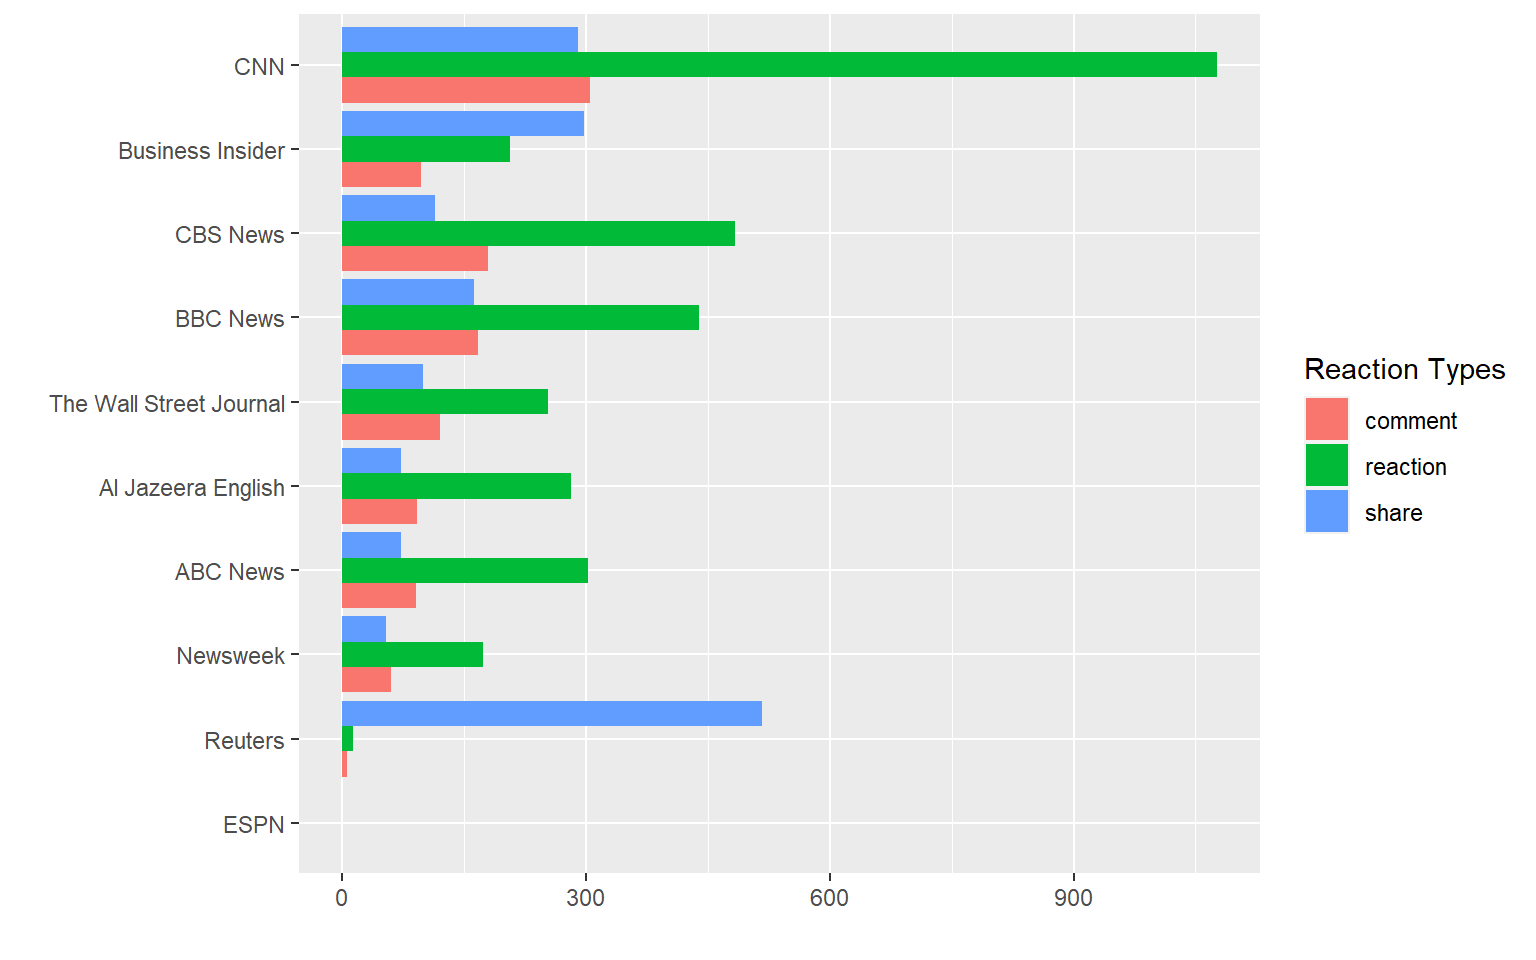
\includegraphics{index_files/figure-latex/unnamed-chunk-4-1} 

}

\caption{Figure 1 - Average number of reaction types per article}\label{fig:unnamed-chunk-4}
\end{figure}

Some really interesting observations to take here. Reuters users are
much more likely to share an article, but otherwise there is a defined
pattern where a \texttt{reaction} is the common engagement type,
followed by \texttt{comments} and then \texttt{shares}. Additionally,
CNN appears to be the most popular amongst the others.

\hypertarget{data-wrangling}{%
\subparagraph{\texorpdfstring{\textbf{Data
Wrangling}}{Data Wrangling}}\label{data-wrangling}}

We will start by doing some data cleansing and will remove the ``460.0''
as the results inferred here would be statistically invalid due to
having only one occurrence.

\begin{Shaded}
\begin{Highlighting}[]
\FunctionTok{library}\NormalTok{(janitor)}

\NormalTok{articles }\OtherTok{\textless{}{-}}\NormalTok{ articles }\SpecialCharTok{\%\textgreater{}\%}
            \FunctionTok{clean\_names}\NormalTok{() }\SpecialCharTok{\%\textgreater{}\%}
            \FunctionTok{rename}\NormalTok{(}\AttributeTok{id =}\NormalTok{ x1) }\SpecialCharTok{\%\textgreater{}\%}
            \FunctionTok{mutate}\NormalTok{(}\AttributeTok{id =} \FunctionTok{row\_number}\NormalTok{()) }\SpecialCharTok{\%\textgreater{}\%}
            \FunctionTok{filter}\NormalTok{(source\_name }\SpecialCharTok{!=} \StringTok{"460.0"}\NormalTok{)}
\end{Highlighting}
\end{Shaded}

Now we'll create a unique article id by newspaper agency.

\begin{Shaded}
\begin{Highlighting}[]
\NormalTok{clean\_articles }\OtherTok{\textless{}{-}}\NormalTok{ articles }\SpecialCharTok{\%\textgreater{}\%}
                 \FunctionTok{group\_by}\NormalTok{(source\_name) }\SpecialCharTok{\%\textgreater{}\%}
                 \FunctionTok{mutate}\NormalTok{(}\AttributeTok{reference =} \FunctionTok{row\_number}\NormalTok{()) }\SpecialCharTok{\%\textgreater{}\%}
                 \FunctionTok{ungroup}\NormalTok{() }\SpecialCharTok{\%\textgreater{}\%}
                 \FunctionTok{mutate}\NormalTok{(}\AttributeTok{article\_id =} \FunctionTok{paste0}\NormalTok{(source\_name, }\StringTok{"\_"}\NormalTok{, reference)) }\SpecialCharTok{\%\textgreater{}\%}
                 \FunctionTok{select}\NormalTok{(}\SpecialCharTok{{-}}\NormalTok{reference)}

\FunctionTok{str}\NormalTok{(clean\_articles[}\DecValTok{1}\NormalTok{,])}
\end{Highlighting}
\end{Shaded}

\begin{verbatim}
## tibble [1 x 16] (S3: tbl_df/tbl/data.frame)
##  $ id                             : int 1
##  $ source_id                      : Factor w/ 13 levels "1","abc-news",..: 10
##  $ source_name                    : Factor w/ 13 levels "460.0","ABC News",..: 10
##  $ author                         : chr "Reuters Editorial"
##  $ title                          : chr "NTSB says Autopilot engaged in 2018 California Tesla crash"
##  $ description                    : chr "The National Transportation Safety Board said Tuesday a Tesla Model S was in Autopilot mode when it struck a fi"| __truncated__
##  $ url                            : chr "https://www.reuters.com/article/us-tesla-crash-idUSKCN1VO22E"
##  $ url_to_image                   : chr "https://s4.reutersmedia.net/resources/r/?m=02&d=20190903&t=2&i=1425817142&w=1200&r=LYNXNPEF821HS"
##  $ published_at                   : POSIXct[1:1], format: "2019-09-03 16:22:20"
##  $ content                        : chr "WASHINGTON (Reuters) - The National Transportation Safety Board said Tuesday a Tesla Model S was in Autopilot m"| __truncated__
##  $ top_article                    : num 0
##  $ engagement_reaction_count      : num 0
##  $ engagement_comment_count       : num 0
##  $ engagement_share_count         : num 2528
##  $ engagement_comment_plugin_count: num 0
##  $ article_id                     : chr "Reuters_1"
\end{verbatim}

\hypertarget{tokenization}{%
\subparagraph{\texorpdfstring{\textbf{Tokenization}}{Tokenization}}\label{tokenization}}

Many of the principles used below have been utilized by the amazing
\texttt{tidytext} package which has been authored by both
\texttt{Silge\ and\ Robinson}. We will now arrange the dataset into a
one-token-per-row format using the \texttt{unnest\_tokens()} verb.

\begin{Shaded}
\begin{Highlighting}[]
\FunctionTok{library}\NormalTok{(tidytext)}

\NormalTok{tidy\_articles }\OtherTok{\textless{}{-}}\NormalTok{ clean\_articles }\SpecialCharTok{\%\textgreater{}\%}
                 \FunctionTok{unnest\_tokens}\NormalTok{(word, description) }
\end{Highlighting}
\end{Shaded}

We will then anti-join stop words, which are common language fillers
such as \texttt{the} and \texttt{a} (Silge and Robinson) so our text
analysis is based on meaningful words.

\begin{Shaded}
\begin{Highlighting}[]
\FunctionTok{data}\NormalTok{(stop\_words)}

\NormalTok{tidy\_articles }\OtherTok{\textless{}{-}}\NormalTok{ tidy\_articles }\SpecialCharTok{\%\textgreater{}\%}
                  \FunctionTok{anti\_join}\NormalTok{(stop\_words)}

\NormalTok{tidy\_articles }\SpecialCharTok{\%\textgreater{}\%}
  \FunctionTok{count}\NormalTok{(word, }\AttributeTok{sort =} \ConstantTok{TRUE}\NormalTok{)}
\end{Highlighting}
\end{Shaded}

\begin{verbatim}
## # A tibble: 21,960 x 2
##    word          n
##    <chr>     <int>
##  1 news       1614
##  2 world       857
##  3 president   841
##  4 national    658
##  5 trump       614
##  6 top         596
##  7 u.s         593
##  8 video       509
##  9 online      480
## 10 coverage    449
## # ... with 21,950 more rows
\end{verbatim}

\hypertarget{text-correlation-analysis}{%
\subparagraph{\texorpdfstring{\textbf{Text correlation
analysis}}{Text correlation analysis}}\label{text-correlation-analysis}}

Now we create \texttt{prop}, which summarizes the proportion each word
has has been mentioned by each respective News provider.

\begin{Shaded}
\begin{Highlighting}[]
\NormalTok{prop }\OtherTok{\textless{}{-}}\NormalTok{ tidy\_articles }\SpecialCharTok{\%\textgreater{}\%}
        \FunctionTok{count}\NormalTok{(word, source\_name, }\AttributeTok{sort =} \ConstantTok{TRUE}\NormalTok{) }\SpecialCharTok{\%\textgreater{}\%}
        \FunctionTok{group\_by}\NormalTok{(source\_name) }\SpecialCharTok{\%\textgreater{}\%}
        \FunctionTok{mutate}\NormalTok{(}\AttributeTok{proportion =}\NormalTok{ n }\SpecialCharTok{/} \FunctionTok{sum}\NormalTok{(n)) }\SpecialCharTok{\%\textgreater{}\%}
        \FunctionTok{ungroup}\NormalTok{() }\SpecialCharTok{\%\textgreater{}\%}
        \FunctionTok{select}\NormalTok{(}\SpecialCharTok{{-}}\NormalTok{n)}
\end{Highlighting}
\end{Shaded}

We then filter our newly created dataset for \texttt{Reuters} and use
that to depict a visual representation of the words that more likely to
mentioned to be mentioned by \texttt{Reuters} (i.e.~have a higher
proportion) vs.~words that are less likely to be mentioned (i.e.~having
a lower proportion). A lower proportion will indicate that there is a
higher possibility of occurrence by the other News providers.

\begin{Shaded}
\begin{Highlighting}[]
\NormalTok{prop\_reuters }\OtherTok{\textless{}{-}}\NormalTok{ prop }\SpecialCharTok{\%\textgreater{}\%}
                \FunctionTok{filter}\NormalTok{(source\_name }\SpecialCharTok{==} \StringTok{"Reuters"}\NormalTok{) }\SpecialCharTok{\%\textgreater{}\%}
                \FunctionTok{select}\NormalTok{(word, proportion) }\SpecialCharTok{\%\textgreater{}\%}
                \FunctionTok{rename}\NormalTok{(}\AttributeTok{Reuters =}\NormalTok{ proportion)}
\end{Highlighting}
\end{Shaded}

Before we visualise our results, we'll need to \texttt{left\_join()} the
original proportions to allow for a comparison as the
\texttt{prop\_reuters} dataset doesn't include these.

\begin{Shaded}
\begin{Highlighting}[]
\NormalTok{tidy\_prop }\OtherTok{\textless{}{-}}\NormalTok{ prop }\SpecialCharTok{\%\textgreater{}\%}
  \FunctionTok{left\_join}\NormalTok{(prop\_reuters, }\AttributeTok{by =} \FunctionTok{c}\NormalTok{(}\StringTok{"word"}\NormalTok{))}
\end{Highlighting}
\end{Shaded}

Now we are able to visualise our results\ldots{}

\begin{Shaded}
\begin{Highlighting}[]
\FunctionTok{library}\NormalTok{(scales)}

\FunctionTok{ggplot}\NormalTok{(tidy\_prop, }\FunctionTok{aes}\NormalTok{(}\AttributeTok{x =}\NormalTok{ proportion, }\AttributeTok{y =} \StringTok{\textasciigrave{}}\AttributeTok{Reuters}\StringTok{\textasciigrave{}}\NormalTok{, }
                      \AttributeTok{color =} \FunctionTok{abs}\NormalTok{(}\StringTok{\textasciigrave{}}\AttributeTok{Reuters}\StringTok{\textasciigrave{}} \SpecialCharTok{{-}}\NormalTok{ proportion))) }\SpecialCharTok{+}
  \FunctionTok{geom\_abline}\NormalTok{(}\AttributeTok{color =} \StringTok{"gray40"}\NormalTok{, }\AttributeTok{lty =} \DecValTok{2}\NormalTok{) }\SpecialCharTok{+}
  \FunctionTok{geom\_jitter}\NormalTok{(}\AttributeTok{alpha =} \FloatTok{0.1}\NormalTok{, }\AttributeTok{size =} \FloatTok{2.5}\NormalTok{, }\AttributeTok{width =} \FloatTok{0.3}\NormalTok{, }\AttributeTok{height =} \FloatTok{0.3}\NormalTok{) }\SpecialCharTok{+}
  \FunctionTok{geom\_text}\NormalTok{(}\FunctionTok{aes}\NormalTok{(}\AttributeTok{label =}\NormalTok{ word), }\AttributeTok{check\_overlap =} \ConstantTok{TRUE}\NormalTok{, }\AttributeTok{vjust =} \FloatTok{1.5}\NormalTok{) }\SpecialCharTok{+}
  \FunctionTok{scale\_x\_log10}\NormalTok{(}\AttributeTok{labels =} \FunctionTok{percent\_format}\NormalTok{()) }\SpecialCharTok{+}
  \FunctionTok{scale\_y\_log10}\NormalTok{(}\AttributeTok{labels =} \FunctionTok{percent\_format}\NormalTok{()) }\SpecialCharTok{+}
  \FunctionTok{scale\_color\_gradient}\NormalTok{(}\AttributeTok{limits =} \FunctionTok{c}\NormalTok{(}\DecValTok{0}\NormalTok{, }\FloatTok{0.001}\NormalTok{), }
                       \AttributeTok{low =} \StringTok{"darkslategray4"}\NormalTok{, }\AttributeTok{high =} \StringTok{"gray75"}\NormalTok{) }\SpecialCharTok{+}
  \FunctionTok{facet\_wrap}\NormalTok{(}\SpecialCharTok{\textasciitilde{}}\NormalTok{source\_name, }\AttributeTok{ncol =} \DecValTok{3}\NormalTok{) }\SpecialCharTok{+}
  \FunctionTok{theme}\NormalTok{(}\AttributeTok{legend.position=}\StringTok{"none"}\NormalTok{) }\SpecialCharTok{+}
  \FunctionTok{labs}\NormalTok{(}\AttributeTok{y =} \StringTok{"Reuters proportions"}\NormalTok{, }\AttributeTok{x =} \ConstantTok{NULL}\NormalTok{)}
\end{Highlighting}
\end{Shaded}

\begin{figure}

{\centering 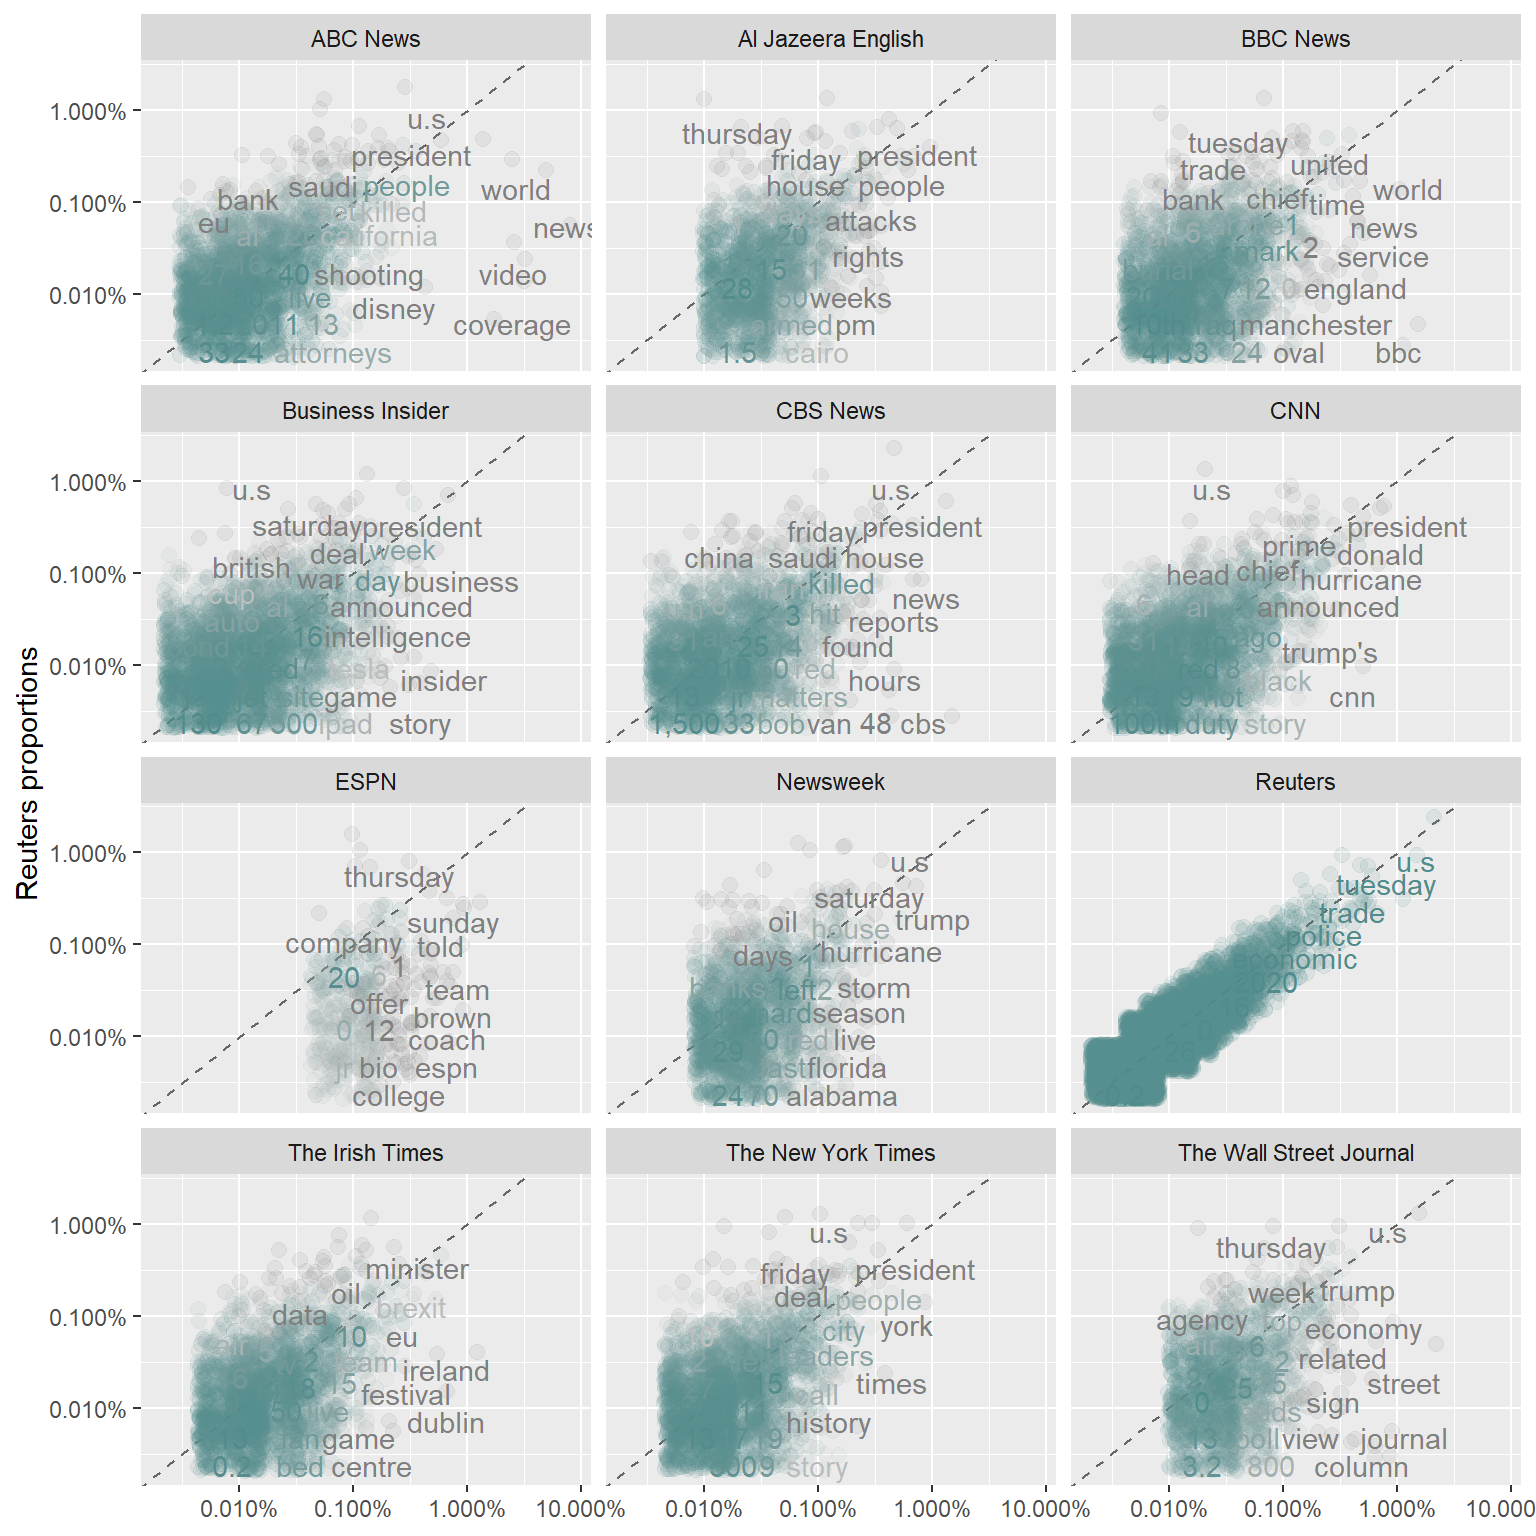
\includegraphics{index_files/figure-latex/unnamed-chunk-12-1} 

}

\caption{Figure 2 - Comparing word freqencies of Reuters against other News services}\label{fig:unnamed-chunk-12}
\end{figure}

\emph{Interesting!} We can tell straight from the graphs that ESPN has
the lowest correlation against Reuters. This was expected, since
\texttt{ESPN}'s coverage is focused on sports-related content unlike the
other source providers which cover broader topic areas.

We will now quantify this correlation against \texttt{ESPN} to
substantiate our results and translate these into numbers using
\texttt{Pearson\textquotesingle{}s\ correlation} by calculating
statistic through \texttt{cor.test}.

\begin{Shaded}
\begin{Highlighting}[]
\FunctionTok{cor.test}\NormalTok{(}\AttributeTok{data =}\NormalTok{ tidy\_prop[tidy\_prop}\SpecialCharTok{$}\NormalTok{source\_name }\SpecialCharTok{==} \StringTok{"ESPN"}\NormalTok{,], }\SpecialCharTok{\textasciitilde{}}\NormalTok{ proportion }\SpecialCharTok{+} \StringTok{\textasciigrave{}}\AttributeTok{Reuters}\StringTok{\textasciigrave{}}\NormalTok{)}
\end{Highlighting}
\end{Shaded}

\begin{verbatim}
## 
##  Pearson's product-moment correlation
## 
## data:  proportion and Reuters
## t = 4.1785, df = 452, p-value = 3.524e-05
## alternative hypothesis: true correlation is not equal to 0
## 95 percent confidence interval:
##  0.1026415 0.2799119
## sample estimates:
##       cor 
## 0.1928498
\end{verbatim}

Now, we'll write a function to pull \texttt{Reuters} correlations
against all other sources and test again for \texttt{ESPN}.

\begin{Shaded}
\begin{Highlighting}[]
\NormalTok{correlation\_function }\OtherTok{\textless{}{-}} \ControlFlowTok{function}\NormalTok{(x) \{}
\FunctionTok{cor.test}\NormalTok{(}\AttributeTok{data =}\NormalTok{ tidy\_prop[tidy\_prop}\SpecialCharTok{$}\NormalTok{source\_name }\SpecialCharTok{==}\NormalTok{ x,], }\SpecialCharTok{\textasciitilde{}}\NormalTok{ proportion }\SpecialCharTok{+} \StringTok{\textasciigrave{}}\AttributeTok{Reuters}\StringTok{\textasciigrave{}}\NormalTok{)}
\NormalTok{\}}

\NormalTok{source\_list }\OtherTok{\textless{}{-}} \FunctionTok{as.vector}\NormalTok{(}\FunctionTok{unique}\NormalTok{(tidy\_prop}\SpecialCharTok{$}\NormalTok{source\_name))}

\NormalTok{correlation\_list }\OtherTok{\textless{}{-}} \FunctionTok{map}\NormalTok{(source\_list, correlation\_function) }\SpecialCharTok{\%\textgreater{}\%}
                    \FunctionTok{setNames}\NormalTok{(source\_list)}

\NormalTok{correlation\_list}\SpecialCharTok{$}\NormalTok{ESPN}
\end{Highlighting}
\end{Shaded}

\begin{verbatim}
## 
##  Pearson's product-moment correlation
## 
## data:  proportion and Reuters
## t = 4.1785, df = 452, p-value = 3.524e-05
## alternative hypothesis: true correlation is not equal to 0
## 95 percent confidence interval:
##  0.1026415 0.2799119
## sample estimates:
##       cor 
## 0.1928498
\end{verbatim}

\emph{Awesome!} We derived the exact same correlation but using a
function. We can now plot \texttt{Reuters} correlations against the
other News source providers.

\begin{Shaded}
\begin{Highlighting}[]
\FunctionTok{library}\NormalTok{(reshape2)}
\FunctionTok{library}\NormalTok{(forcats)}

\NormalTok{correlation\_df }\OtherTok{\textless{}{-}} \FunctionTok{melt}\NormalTok{(}\FunctionTok{lapply}\NormalTok{(correlation\_list, }\StringTok{\textasciigrave{}}\AttributeTok{[}\StringTok{\textasciigrave{}}\NormalTok{, }\FunctionTok{c}\NormalTok{(}\StringTok{\textquotesingle{}estimate\textquotesingle{}}\NormalTok{, }\StringTok{\textquotesingle{}p.value\textquotesingle{}}\NormalTok{)))}

\NormalTok{tidy\_correlations }\OtherTok{\textless{}{-}}\NormalTok{ correlation\_df }\SpecialCharTok{\%\textgreater{}\%}
                     \FunctionTok{filter}\NormalTok{(L2 }\SpecialCharTok{==} \StringTok{"estimate"}\NormalTok{, L1 }\SpecialCharTok{!=} \StringTok{"Reuters"}\NormalTok{) }\SpecialCharTok{\%\textgreater{}\%}
                     \FunctionTok{rename}\NormalTok{(}\AttributeTok{source\_name =}\NormalTok{ L1) }\SpecialCharTok{\%\textgreater{}\%}
                     \FunctionTok{select}\NormalTok{(}\SpecialCharTok{{-}}\NormalTok{L2) }\SpecialCharTok{\%\textgreater{}\%}
                     \FunctionTok{ggplot}\NormalTok{(}\FunctionTok{aes}\NormalTok{(}\FunctionTok{fct\_reorder}\NormalTok{(source\_name, value),value)) }\SpecialCharTok{+}
                     \FunctionTok{geom\_col}\NormalTok{() }\SpecialCharTok{+} 
                     \FunctionTok{coord\_flip}\NormalTok{() }\SpecialCharTok{+} 
                     \FunctionTok{xlab}\NormalTok{(}\ConstantTok{NULL}\NormalTok{) }\SpecialCharTok{+}
                     \FunctionTok{ylab}\NormalTok{(}\StringTok{""}\NormalTok{)}

\NormalTok{tidy\_correlations}
\end{Highlighting}
\end{Shaded}

\begin{figure}

{\centering 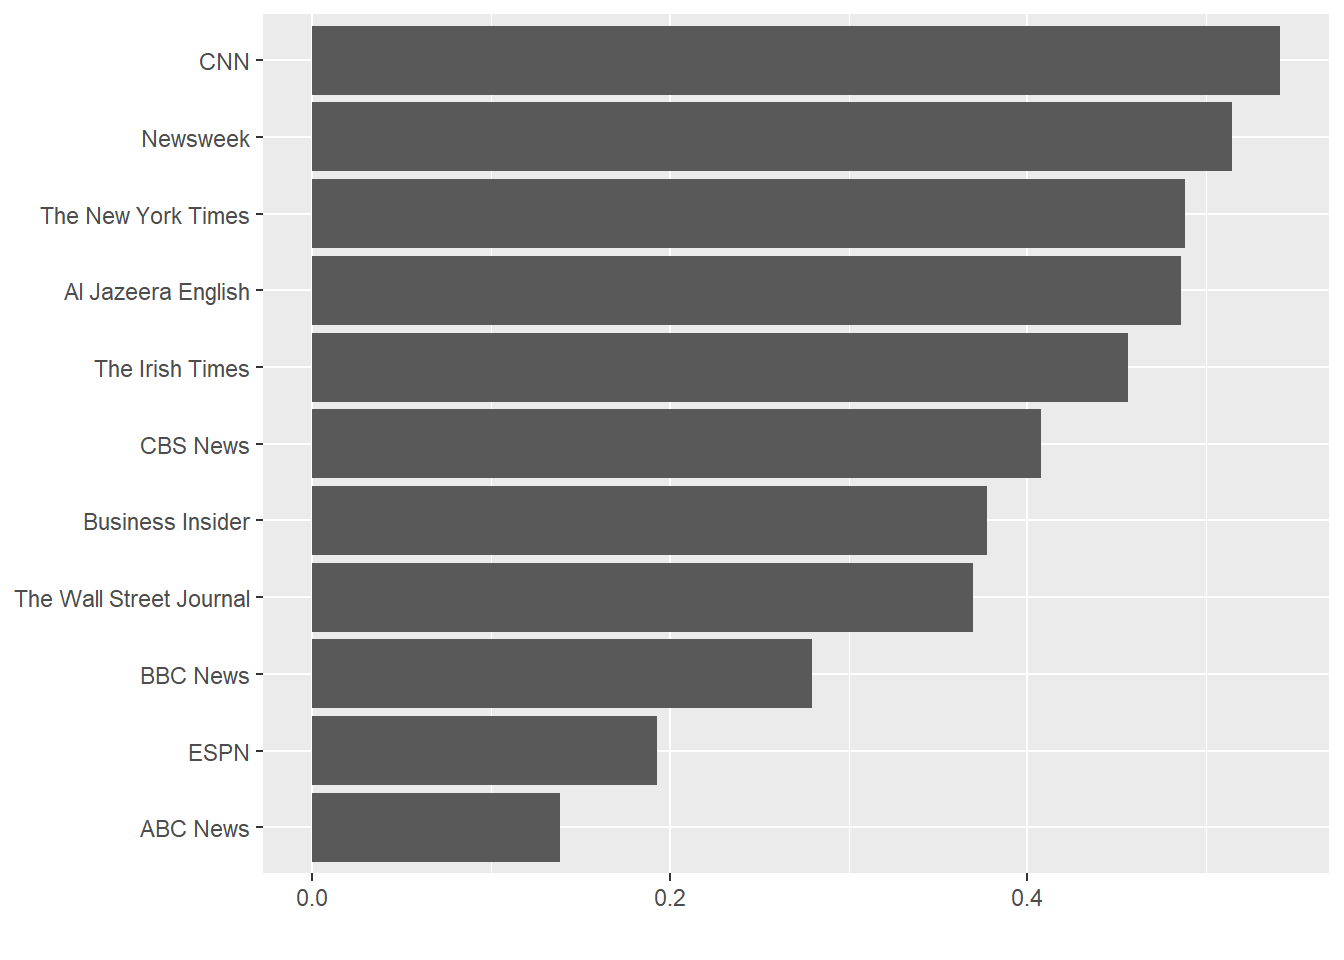
\includegraphics{index_files/figure-latex/unnamed-chunk-15-1} 

}

\caption{Figure 3 - Reuters text correlation with other News sources}\label{fig:unnamed-chunk-15}
\end{figure}

Interesting to see \texttt{ABC} news with even lower correlation than
\texttt{ESPN}'s. A closer look at the plot above shows the words
\emph{world}, \emph{news}, \emph{video}, \emph{coverage} as clear
outliers causing ABC News to have this awfully low correlation even
though \texttt{ESPN}'s content is much more diverse.

\textbf{Note}: Our analysis results would have been much different had
we used the \texttt{content} column in the description dataset. However,
because results have been truncated to 260 characters we believe it
would be very difficult to infer meaningful relationships through
missing content, and therefore have based our analysis on the
\texttt{description} column which provides an excellent summary of the
article events, and is a lot more detailed than the \texttt{title}
column.

\hypertarget{topic-modeling}{%
\subsubsection{\texorpdfstring{\textbf{Topic
modeling}}{Topic modeling}}\label{topic-modeling}}

Now we move on to \texttt{topic\ modeling}, where our goal is to show
you the various topic clusters within the \texttt{articles} dataset by
article. We start by arranging our dataset into a tidy format.

\begin{Shaded}
\begin{Highlighting}[]
\NormalTok{wordsbyArticle }\OtherTok{\textless{}{-}}\NormalTok{ tidy\_articles }\SpecialCharTok{\%\textgreater{}\%}
                   \FunctionTok{count}\NormalTok{(article\_id, word, }\AttributeTok{sort =} \ConstantTok{TRUE}\NormalTok{) }

\NormalTok{wordsbyArticle}
\end{Highlighting}
\end{Shaded}

\begin{verbatim}
## # A tibble: 142,737 x 3
##    article_id           word       n
##    <chr>                <chr>  <int>
##  1 Business Insider_688 iphone     6
##  2 Business Insider_461 iphone     5
##  3 Business Insider_477 iphone     5
##  4 Business Insider_486 iphone     5
##  5 Business Insider_561 11         5
##  6 Business Insider_561 iphone     5
##  7 Business Insider_640 litter     5
##  8 Business Insider_805 coca       5
##  9 Business Insider_805 cola       5
## 10 CNN_621              iphone     5
## # ... with 142,727 more rows
\end{verbatim}

We will now transform this into a dfm object using the
\texttt{cast\_dfm()} function from using the \texttt{tidytext}package
(Silge and Robinson). A dfm-class object is a sparse matrix
representation of the counts of features by document, and is needed to
apply the \texttt{stm} function, which is a method of unsupervised
classification widely accepted as suitable topic modeling method.

Due to the excruciating amount of time needed to knit the document with
the \texttt{stm}, we have opted to save the file into our workspace to
make the knitting process much smoother and quicker ! We have also saved
the seed number for reproducibility.

\begin{Shaded}
\begin{Highlighting}[]
\FunctionTok{library}\NormalTok{(tm)}
\FunctionTok{library}\NormalTok{(quanteda)}
\FunctionTok{library}\NormalTok{(stm)}

\NormalTok{articles\_dfm }\OtherTok{\textless{}{-}}\NormalTok{ wordsbyArticle }\SpecialCharTok{\%\textgreater{}\%}
  \FunctionTok{cast\_dfm}\NormalTok{(article\_id, word, n)}

\FunctionTok{set.seed}\NormalTok{(}\DecValTok{2021}\NormalTok{)}
\NormalTok{articles\_lda }\OtherTok{\textless{}{-}} \FunctionTok{stm}\NormalTok{(articles\_dfm, }\AttributeTok{K=}\DecValTok{6}\NormalTok{, }\AttributeTok{init.type =} \StringTok{"LDA"}\NormalTok{)}
\FunctionTok{saveRDS}\NormalTok{(articles\_lda, }\AttributeTok{file =} \StringTok{"articles\_lda.RDS"}\NormalTok{)}
\NormalTok{rownames\_dfm }\OtherTok{\textless{}{-}} \FunctionTok{rownames}\NormalTok{(articles\_dfm)}
\FunctionTok{saveRDS}\NormalTok{(rownames\_dfm, }\AttributeTok{file =} \StringTok{"rownames\_dfm.RDS"}\NormalTok{)}
\end{Highlighting}
\end{Shaded}

\begin{Shaded}
\begin{Highlighting}[]
\NormalTok{articles\_lda }\OtherTok{\textless{}{-}} \FunctionTok{readRDS}\NormalTok{(}\AttributeTok{file =} \StringTok{"articles\_lda.RDS"}\NormalTok{)}
\NormalTok{rownames\_dfm  }\OtherTok{\textless{}{-}} \FunctionTok{readRDS}\NormalTok{(}\AttributeTok{file =} \StringTok{"rownames\_dfm.RDS"}\NormalTok{)}
\end{Highlighting}
\end{Shaded}

Now, that we've successfully run the topic models, we will group these
into different categories. To avoid repeating the graph twice, we will
label these prior to visualising the top 10 words from each of the 6
topics.

\begin{Shaded}
\begin{Highlighting}[]
\NormalTok{article\_topics }\OtherTok{\textless{}{-}} \FunctionTok{tidy}\NormalTok{(articles\_lda, }\AttributeTok{matrix =} \StringTok{"beta"}\NormalTok{)}

\NormalTok{topic\_theme }\OtherTok{\textless{}{-}}\NormalTok{ article\_topics }\SpecialCharTok{\%\textgreater{}\%}
  \FunctionTok{group\_by}\NormalTok{(topic) }\SpecialCharTok{\%\textgreater{}\%}
  \FunctionTok{slice\_max}\NormalTok{(beta, }\AttributeTok{n =} \DecValTok{10}\NormalTok{) }\SpecialCharTok{\%\textgreater{}\%}
  \FunctionTok{ungroup}\NormalTok{() }\SpecialCharTok{\%\textgreater{}\%}
  \FunctionTok{arrange}\NormalTok{(topic, }\SpecialCharTok{{-}}\NormalTok{beta)}

\NormalTok{topic\_categories }\OtherTok{\textless{}{-}} \FunctionTok{tibble}\NormalTok{(}\AttributeTok{topic =} \DecValTok{1}\SpecialCharTok{:}\DecValTok{6}\NormalTok{, }\AttributeTok{topic\_category =} \FunctionTok{c}\NormalTok{(}\StringTok{"Exclusive content"}\NormalTok{, }\StringTok{"Economy and Trade"}\NormalTok{, }\StringTok{"Climate change"}\NormalTok{, }\StringTok{"US coverage"}\NormalTok{, }\StringTok{"International coverage"}\NormalTok{, }\StringTok{"UK coverage"}\NormalTok{))}

\NormalTok{topic\_theme }\SpecialCharTok{\%\textgreater{}\%}
  \FunctionTok{inner\_join}\NormalTok{(topic\_categories, }\AttributeTok{by =} \FunctionTok{c}\NormalTok{(}\StringTok{"topic"}\NormalTok{)) }\SpecialCharTok{\%\textgreater{}\%}
  \FunctionTok{ggplot}\NormalTok{(}\FunctionTok{aes}\NormalTok{(}\FunctionTok{fct\_reorder}\NormalTok{(term, beta), beta, }\AttributeTok{fill =} \FunctionTok{factor}\NormalTok{(topic\_category))) }\SpecialCharTok{+} 
  \FunctionTok{geom\_col}\NormalTok{(}\AttributeTok{show.legend =} \ConstantTok{FALSE}\NormalTok{) }\SpecialCharTok{+} 
  \FunctionTok{facet\_wrap}\NormalTok{(}\SpecialCharTok{\textasciitilde{}}\NormalTok{topic\_category, }\AttributeTok{scales =} \StringTok{"free"}\NormalTok{) }\SpecialCharTok{+} 
  \FunctionTok{coord\_flip}\NormalTok{() }\SpecialCharTok{+}
  \FunctionTok{ylab}\NormalTok{(}\StringTok{""}\NormalTok{) }\SpecialCharTok{+}
  \FunctionTok{xlab}\NormalTok{(}\StringTok{""}\NormalTok{)}
\end{Highlighting}
\end{Shaded}

\begin{figure}

{\centering 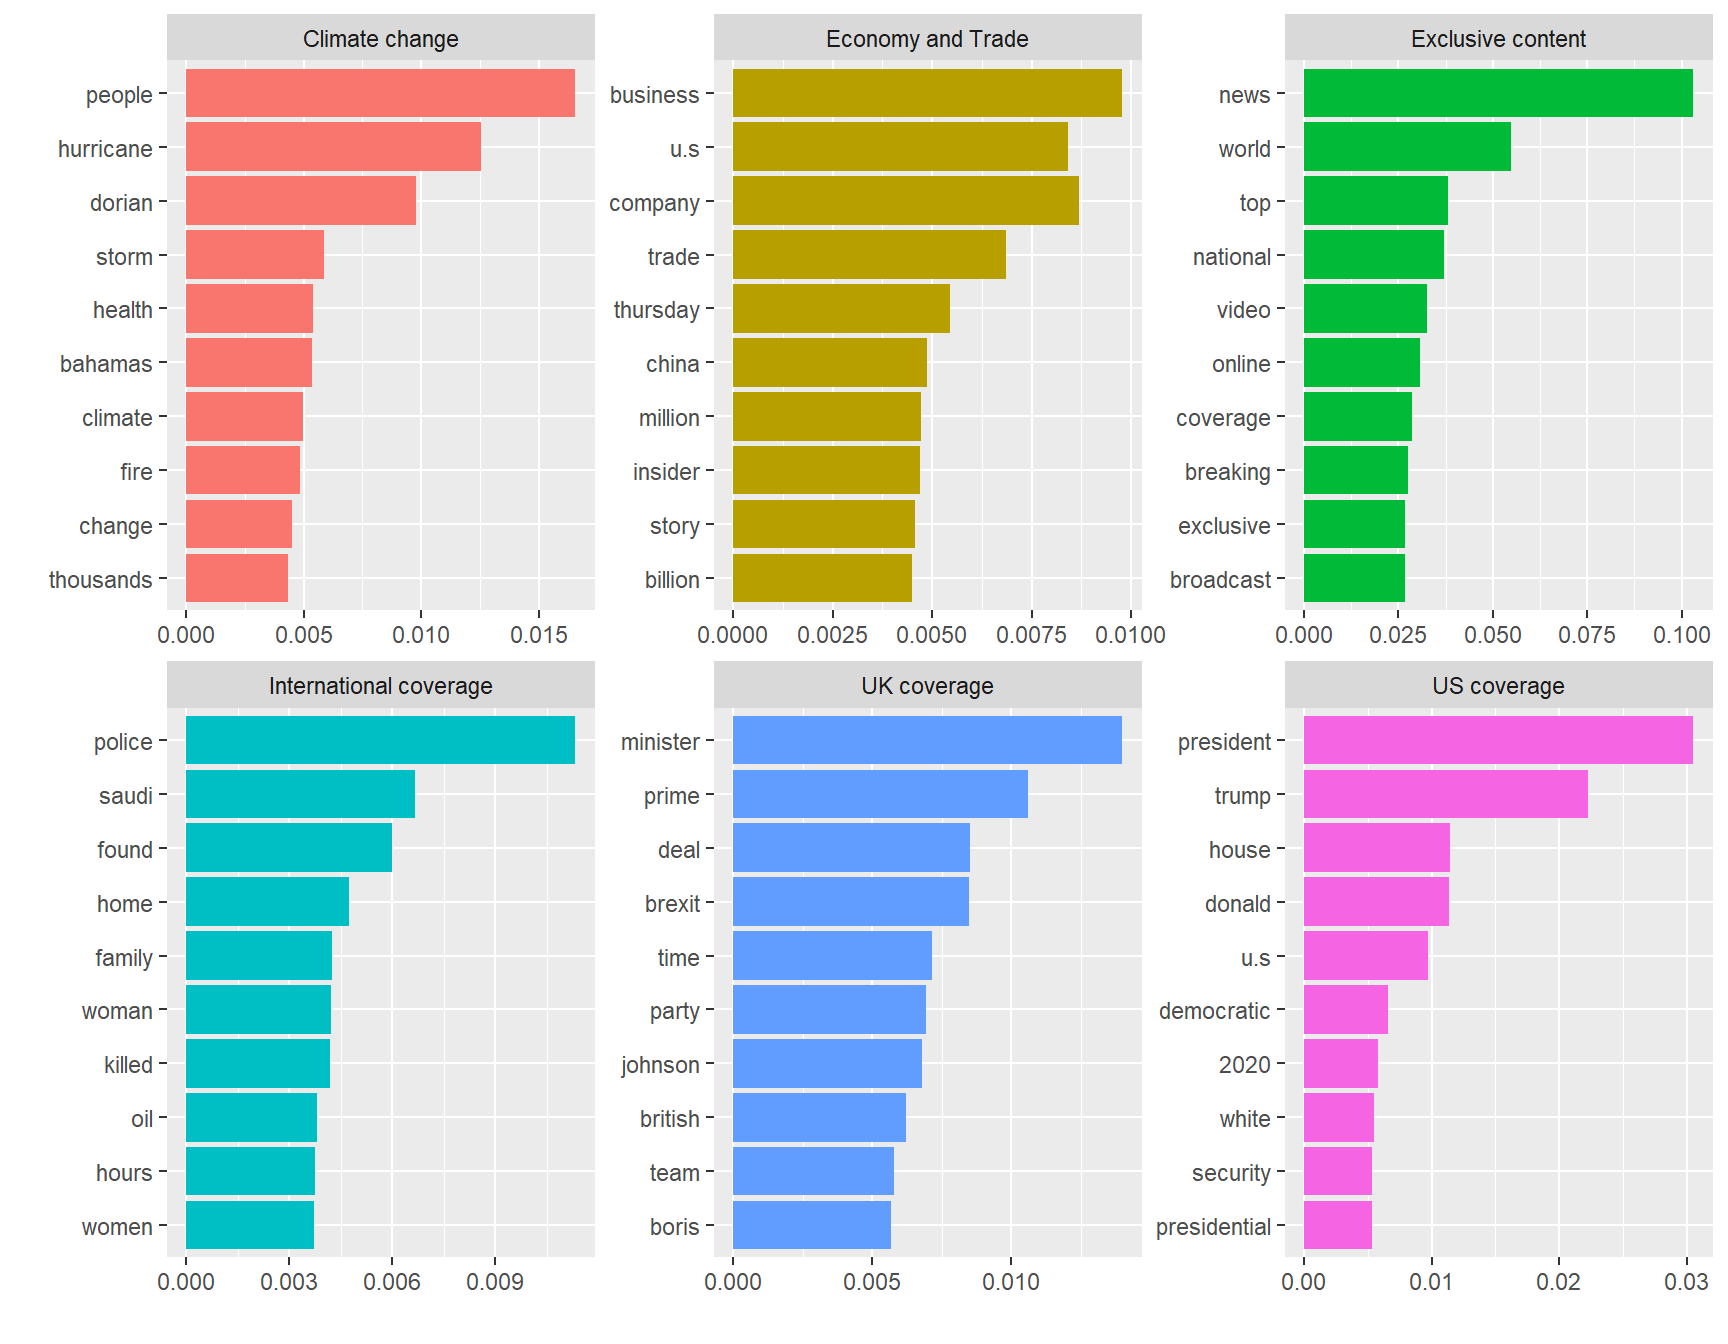
\includegraphics{index_files/figure-latex/unnamed-chunk-19-1} 

}

\caption{Figure 4 - Terms that are most common within each of the six topics}\label{fig:unnamed-chunk-19}
\end{figure}

Even though there is some judgement involved surrounding the
nomenclature of these topic categories, we can clearly distinguish
certain topic areas such as \emph{Economy and Trade}, \emph{Climate
change}, \emph{US coverage}, and \emph{UK coverage}. Other areas such as
\emph{International coverage} are more likely disputed but most probably
accepted to fit a range of other topics. This opens the possibility to
perform topic modelling using a k \textgreater{} 6. Also,
\emph{Exclusive} sounds a bit vague and not well defined but we believe
it is driven by the \texttt{description} column in the dataset being
limited to certain characters. However, for our purposes we will keep
this to examine later on whether exclusive content has a significant
impact on popularity.

Now we'll turn our focus to \texttt{gamma}, which moves away slightly
from a word focus and is an allocation of various topics within a single
document (Silge and Robinson). So in our case, this would be the topics
allocation which each article from our articles dataset (i.e.~allocation
by \texttt{article\_id})

\begin{Shaded}
\begin{Highlighting}[]
\NormalTok{articles\_gamma }\OtherTok{\textless{}{-}} \FunctionTok{tidy}\NormalTok{(articles\_lda, }\AttributeTok{matrix =} \StringTok{"gamma"}\NormalTok{, }\AttributeTok{document\_names =}\NormalTok{ rownames\_dfm)}

\NormalTok{articles\_gamma\_sliced }\OtherTok{\textless{}{-}}\NormalTok{ articles\_gamma }\SpecialCharTok{\%\textgreater{}\%}
  \FunctionTok{group\_by}\NormalTok{(document) }\SpecialCharTok{\%\textgreater{}\%}
  \FunctionTok{slice\_max}\NormalTok{(}\AttributeTok{order\_by =}\NormalTok{ gamma, }\AttributeTok{n=}\DecValTok{1}\NormalTok{) }\SpecialCharTok{\%\textgreater{}\%}
  \FunctionTok{ungroup}\NormalTok{() }\SpecialCharTok{\%\textgreater{}\%}
  \FunctionTok{arrange}\NormalTok{(}\SpecialCharTok{{-}}\NormalTok{gamma) }\SpecialCharTok{\%\textgreater{}\%}
  \FunctionTok{inner\_join}\NormalTok{(topic\_categories) }\SpecialCharTok{\%\textgreater{}\%}
  \FunctionTok{rename}\NormalTok{(}\AttributeTok{article\_id =}\NormalTok{ document)}
  
\NormalTok{articles\_gamma\_sliced }\SpecialCharTok{\%\textgreater{}\%}  
\FunctionTok{separate}\NormalTok{(article\_id, }\FunctionTok{c}\NormalTok{(}\StringTok{\textquotesingle{}source\_name\textquotesingle{}}\NormalTok{, }\StringTok{\textquotesingle{}article\_number\textquotesingle{}}\NormalTok{), }\AttributeTok{sep=}\StringTok{"\_"}\NormalTok{) }\SpecialCharTok{\%\textgreater{}\%}
\FunctionTok{count}\NormalTok{(source\_name, topic, topic\_category) }\SpecialCharTok{\%\textgreater{}\%}
\FunctionTok{ggplot}\NormalTok{(}\FunctionTok{aes}\NormalTok{(source\_name, n, }\AttributeTok{fill =} \FunctionTok{factor}\NormalTok{(topic\_category))) }\SpecialCharTok{+} 
\FunctionTok{geom\_col}\NormalTok{(}\AttributeTok{position =} \StringTok{"fill"}\NormalTok{) }\SpecialCharTok{+} 
\FunctionTok{coord\_flip}\NormalTok{() }\SpecialCharTok{+} 
\FunctionTok{guides}\NormalTok{(}\AttributeTok{fill=}\FunctionTok{guide\_legend}\NormalTok{(}\AttributeTok{title=}\StringTok{"Topic categories"}\NormalTok{)) }\SpecialCharTok{+}
\FunctionTok{ylab}\NormalTok{(}\StringTok{""}\NormalTok{) }\SpecialCharTok{+}
\FunctionTok{xlab}\NormalTok{(}\StringTok{""}\NormalTok{)}
\end{Highlighting}
\end{Shaded}

\begin{figure}

{\centering 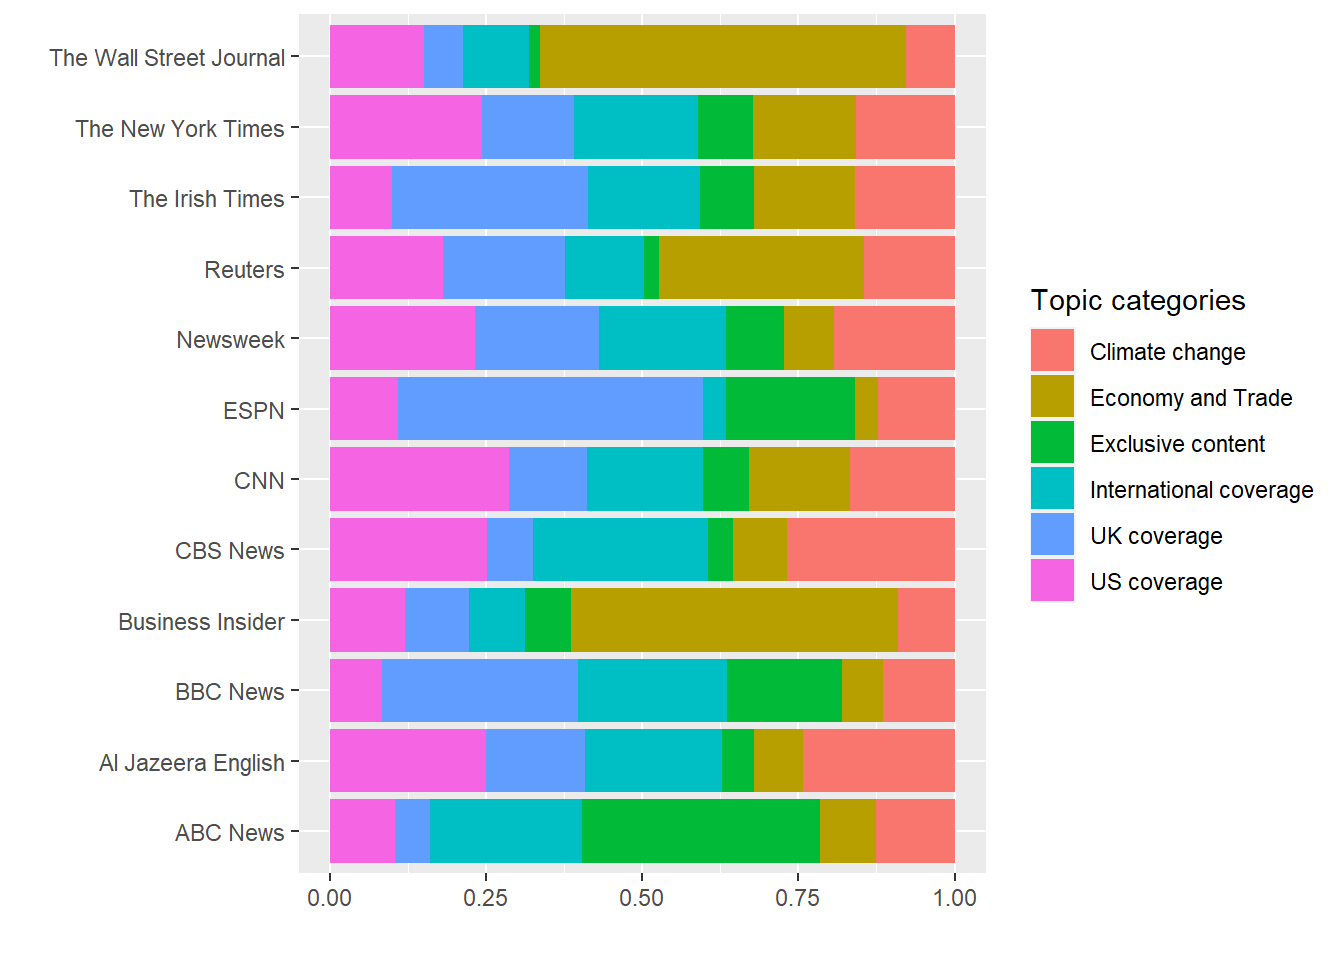
\includegraphics{index_files/figure-latex/unnamed-chunk-20-1} 

}

\caption{Figure 5 - Weighting of our clustered topic categories amongst the various News providers}\label{fig:unnamed-chunk-20}
\end{figure}

The results above are sensical. \texttt{ESPN}'s UK coverage is a result
from the its UK premiere league coverage. \texttt{BBC} obviously has
higher UK coverage than its counterparts. \texttt{WSJ} and the
\texttt{Business\ Insider} are mostly focused on Economy and Trade as
would be expected. \texttt{CNN} understandably has a much higher US
coverage than any of its counterparts.

\hypertarget{sentiment-analysis}{%
\subsubsection{Sentiment Analysis}\label{sentiment-analysis}}

Now we'll perform sentiment analysis using the \texttt{bing} dataset
(Silge and Robinson). This lexicon provides a two-category sentiment
which will be useful for our analysis. Using the \texttt{tidytext}
package, we can obtain this lexicon by calling
\texttt{get\_sentiments()}

\begin{verbatim}
## # A tibble: 6,786 x 2
##    word        sentiment
##    <chr>       <chr>    
##  1 2-faces     negative 
##  2 abnormal    negative 
##  3 abolish     negative 
##  4 abominable  negative 
##  5 abominably  negative 
##  6 abominate   negative 
##  7 abomination negative 
##  8 abort       negative 
##  9 aborted     negative 
## 10 aborts      negative 
## # ... with 6,776 more rows
\end{verbatim}

Here, we'll \texttt{inner\_join} the \texttt{bing} dataset to our tidied
set, thereby eliminating any mismatch in words between these two
datsets. We will also assign a \texttt{sentiment} score based on the
frequency of either positive or negative words within each
\texttt{article\_id}

\begin{Shaded}
\begin{Highlighting}[]
\NormalTok{sentiment\_bing }\OtherTok{\textless{}{-}}\NormalTok{ tidy\_articles }\SpecialCharTok{\%\textgreater{}\%}
  \FunctionTok{inner\_join}\NormalTok{(}\FunctionTok{get\_sentiments}\NormalTok{(}\StringTok{"bing"}\NormalTok{)) }\SpecialCharTok{\%\textgreater{}\%}
  \FunctionTok{count}\NormalTok{(article\_id, source\_name, sentiment) }\SpecialCharTok{\%\textgreater{}\%}
  \FunctionTok{spread}\NormalTok{(sentiment, n, }\AttributeTok{fill =} \DecValTok{0}\NormalTok{) }\SpecialCharTok{\%\textgreater{}\%}
  \FunctionTok{mutate}\NormalTok{(}\AttributeTok{sentiment =}\NormalTok{ positive }\SpecialCharTok{{-}}\NormalTok{ negative)}

\NormalTok{sentiment\_bing}
\end{Highlighting}
\end{Shaded}

\begin{verbatim}
## # A tibble: 7,515 x 5
##    article_id    source_name negative positive sentiment
##    <chr>         <fct>          <dbl>    <dbl>     <dbl>
##  1 ABC News_1    ABC News           4        1        -3
##  2 ABC News_10   ABC News           1        1         0
##  3 ABC News_1001 ABC News           2        2         0
##  4 ABC News_1002 ABC News           1        1         0
##  5 ABC News_1004 ABC News           0        2         2
##  6 ABC News_1005 ABC News           2        0        -2
##  7 ABC News_1006 ABC News           1        0        -1
##  8 ABC News_1007 ABC News           0        1         1
##  9 ABC News_1008 ABC News           1        1         0
## 10 ABC News_1009 ABC News           1        1         0
## # ... with 7,505 more rows
\end{verbatim}

\hypertarget{wordcloud}{%
\subsubsection{Wordcloud}\label{wordcloud}}

Now that we have a tidied dataset, we can plot a wordcloud with the
\texttt{reshape2} and \texttt{wordcloud} packages. We can try to
understand the main sentiment drivers (either positive or negative)
within the whole dateset.

\begin{Shaded}
\begin{Highlighting}[]
\FunctionTok{library}\NormalTok{(reshape2)}
\FunctionTok{library}\NormalTok{(wordcloud)}

\NormalTok{tidy\_articles }\SpecialCharTok{\%\textgreater{}\%}
  \FunctionTok{inner\_join}\NormalTok{(}\FunctionTok{get\_sentiments}\NormalTok{(}\StringTok{"bing"}\NormalTok{)) }\SpecialCharTok{\%\textgreater{}\%}
  \FunctionTok{count}\NormalTok{(word, sentiment, }\AttributeTok{sort =} \ConstantTok{TRUE}\NormalTok{) }\SpecialCharTok{\%\textgreater{}\%}
  \FunctionTok{acast}\NormalTok{(word }\SpecialCharTok{\textasciitilde{}}\NormalTok{ sentiment, }\AttributeTok{value.var =} \StringTok{"n"}\NormalTok{, }\AttributeTok{fill =} \DecValTok{0}\NormalTok{) }\SpecialCharTok{\%\textgreater{}\%}
  \FunctionTok{comparison.cloud}\NormalTok{(}\AttributeTok{colors =} \FunctionTok{c}\NormalTok{(}\StringTok{"gray20"}\NormalTok{,}\StringTok{"gray80"}\NormalTok{), }\AttributeTok{max.words =} \DecValTok{75}\NormalTok{)}
\end{Highlighting}
\end{Shaded}

\begin{figure}

{\centering 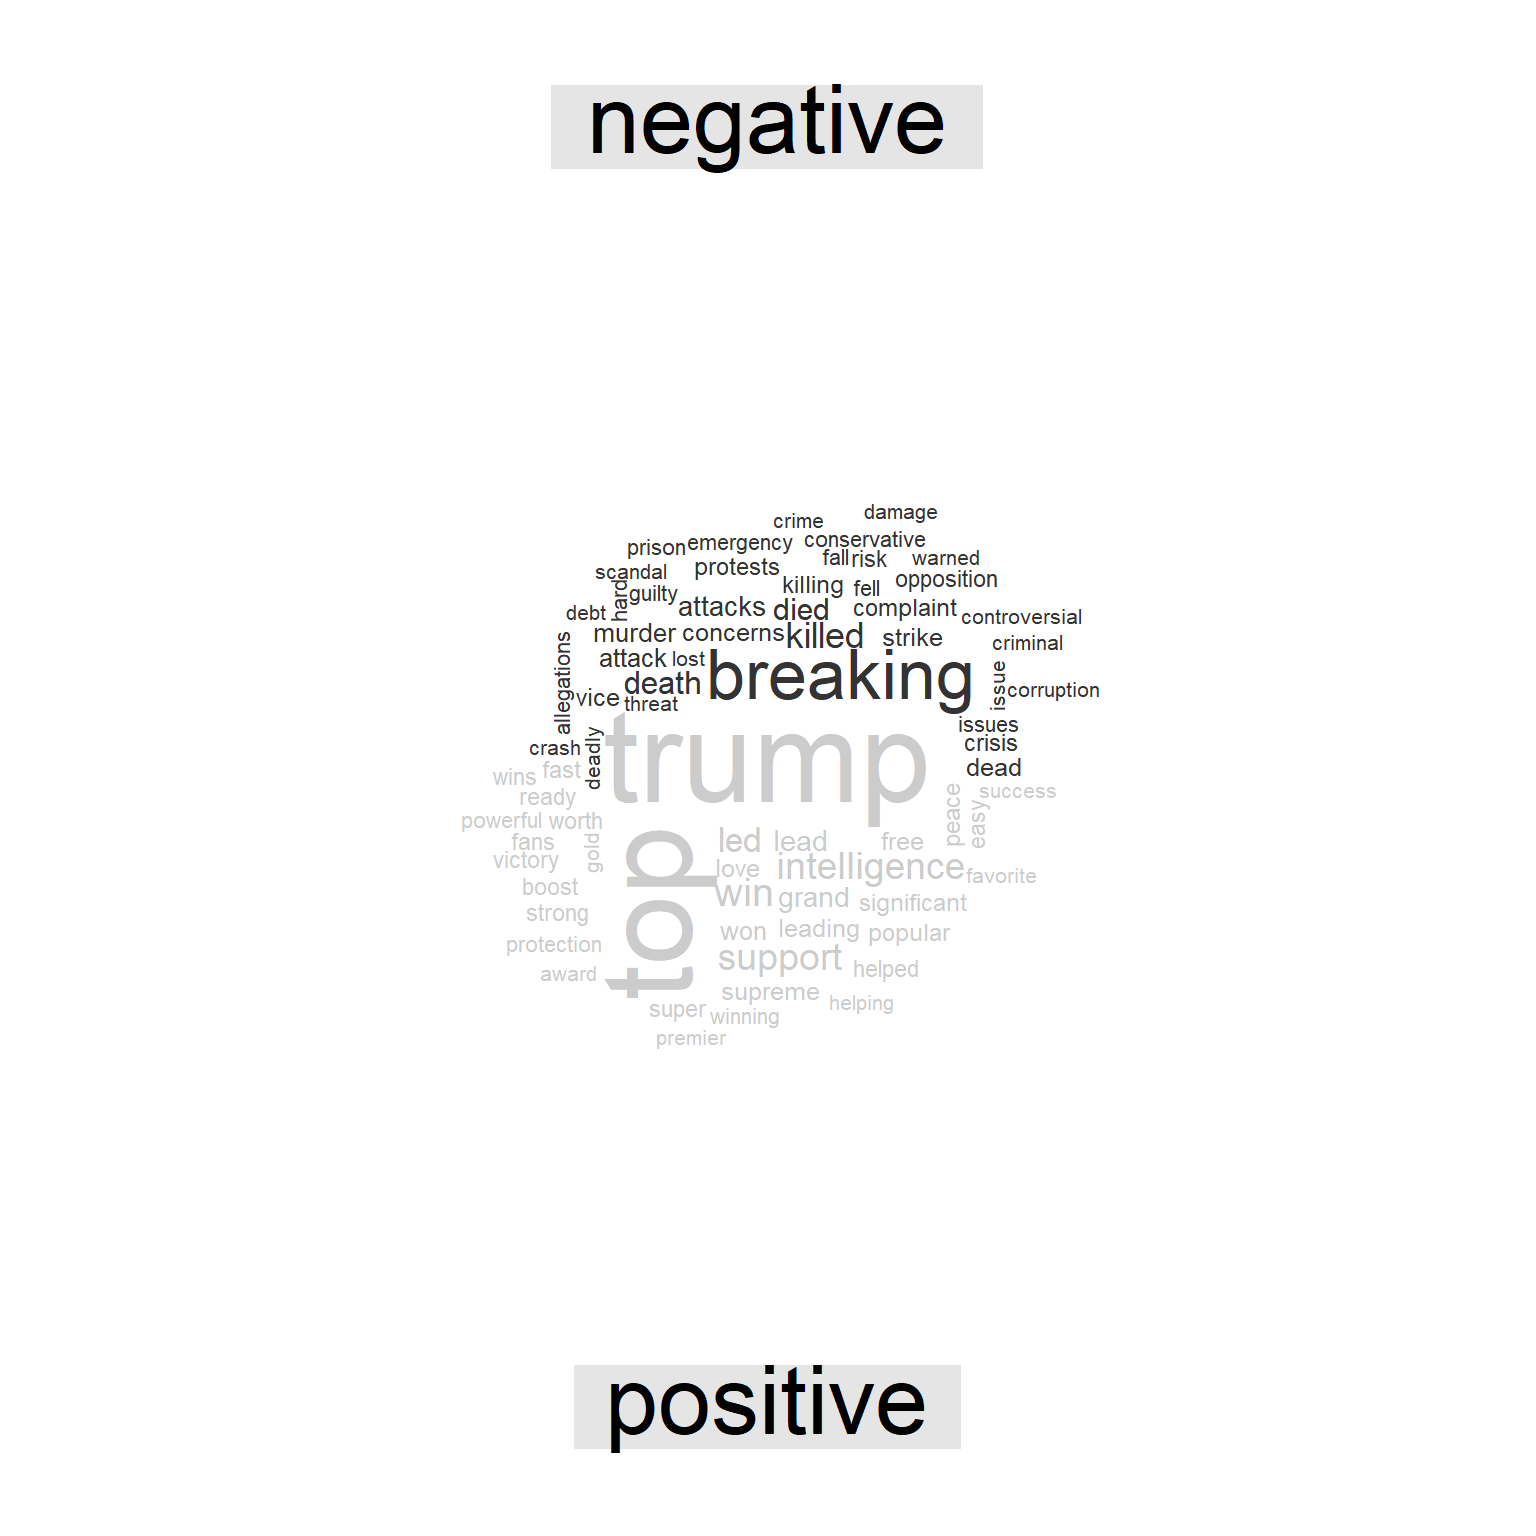
\includegraphics{index_files/figure-latex/unnamed-chunk-23-1} 

}

\caption{Figure 6 - Most common positive and negative words in all articles}\label{fig:unnamed-chunk-23}
\end{figure}

Some of these negative words are distressing, so we can filter our
dataset to \texttt{ESPN} to find more lighthearted indicators of either
negative or positive sentiment.

\begin{Shaded}
\begin{Highlighting}[]
\NormalTok{tidy\_articles }\SpecialCharTok{\%\textgreater{}\%}
  \FunctionTok{inner\_join}\NormalTok{(}\FunctionTok{get\_sentiments}\NormalTok{(}\StringTok{"bing"}\NormalTok{)) }\SpecialCharTok{\%\textgreater{}\%}
  \FunctionTok{count}\NormalTok{(word, sentiment, source\_name, }\AttributeTok{sort =} \ConstantTok{TRUE}\NormalTok{) }\SpecialCharTok{\%\textgreater{}\%}
  \FunctionTok{filter}\NormalTok{(source\_name }\SpecialCharTok{==} \StringTok{"ESPN"}\NormalTok{) }\SpecialCharTok{\%\textgreater{}\%}
  \FunctionTok{acast}\NormalTok{(word }\SpecialCharTok{\textasciitilde{}}\NormalTok{ sentiment, }\AttributeTok{value.var =} \StringTok{"n"}\NormalTok{, }\AttributeTok{fill =} \DecValTok{0}\NormalTok{) }\SpecialCharTok{\%\textgreater{}\%}
  \FunctionTok{comparison.cloud}\NormalTok{(}\AttributeTok{colors =} \FunctionTok{c}\NormalTok{(}\StringTok{"gray20"}\NormalTok{,}\StringTok{"gray80"}\NormalTok{), }\AttributeTok{max.words =} \DecValTok{120}\NormalTok{)}
\end{Highlighting}
\end{Shaded}

\begin{figure}

{\centering 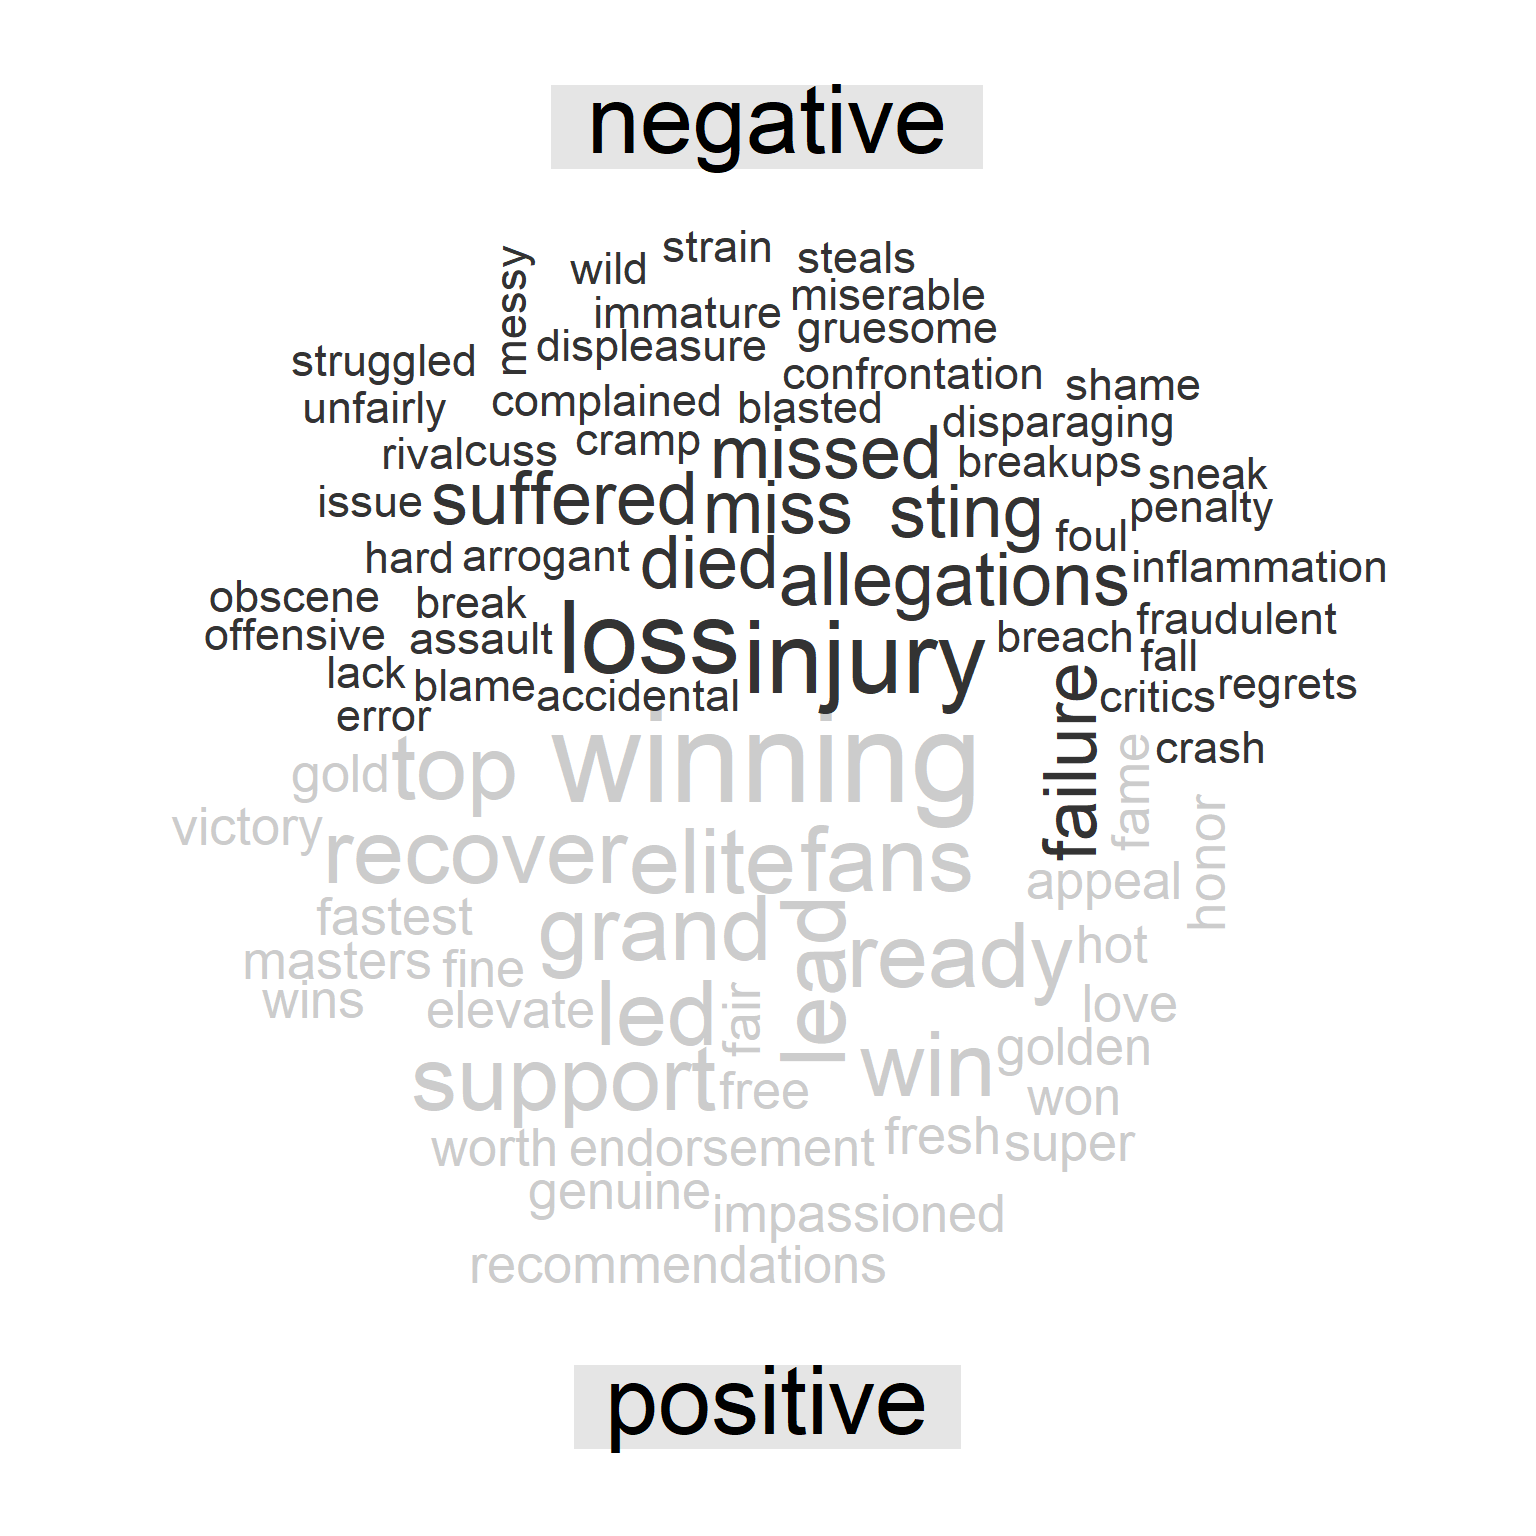
\includegraphics{index_files/figure-latex/unnamed-chunk-24-1} 

}

\caption{Figure 7 - Most common positive and negative words in ESPN articles}\label{fig:unnamed-chunk-24}
\end{figure}

This is more like it, and why people love watching sports!

\hypertarget{term-frequency}{%
\subsubsection{Term Frequency}\label{term-frequency}}

We can also obtain a deeper understanding of the topic areas covered by
each News agency by calculating term frequency, which is the number of
times our words apprear within a document. We will use this concept to
depict the top 15 words most commonly used by each News provider. This
can be performed using the \texttt{bind\_tf\_idf} verb.

\begin{Shaded}
\begin{Highlighting}[]
\NormalTok{article\_words }\OtherTok{\textless{}{-}}\NormalTok{   tidy\_articles }\SpecialCharTok{\%\textgreater{}\%}
                   \FunctionTok{count}\NormalTok{(source\_name, word, }\AttributeTok{sort =} \ConstantTok{TRUE}\NormalTok{)}


\NormalTok{article\_words }\OtherTok{\textless{}{-}}\NormalTok{ article\_words }\SpecialCharTok{\%\textgreater{}\%}
                 \FunctionTok{bind\_tf\_idf}\NormalTok{(word, source\_name, n) }\SpecialCharTok{\%\textgreater{}\%}
                 \FunctionTok{arrange}\NormalTok{(}\SpecialCharTok{{-}}\NormalTok{tf\_idf)}
                 
\NormalTok{article\_words }\SpecialCharTok{\%\textgreater{}\%}
  \FunctionTok{group\_by}\NormalTok{(source\_name) }\SpecialCharTok{\%\textgreater{}\%}
  \FunctionTok{slice\_max}\NormalTok{(tf\_idf, }\AttributeTok{n =} \DecValTok{15}\NormalTok{) }\SpecialCharTok{\%\textgreater{}\%}
\NormalTok{  ungroup }\SpecialCharTok{\%\textgreater{}\%}
  \FunctionTok{ggplot}\NormalTok{(}\FunctionTok{aes}\NormalTok{(word, tf\_idf, }\AttributeTok{fill =}\NormalTok{ source\_name)) }\SpecialCharTok{+}
  \FunctionTok{geom\_col}\NormalTok{(}\AttributeTok{show.legend =} \ConstantTok{FALSE}\NormalTok{) }\SpecialCharTok{+} 
  \FunctionTok{facet\_wrap}\NormalTok{(}\SpecialCharTok{\textasciitilde{}}\NormalTok{source\_name, }\AttributeTok{ncol =} \DecValTok{3}\NormalTok{, }\AttributeTok{scales =} \StringTok{"free"}\NormalTok{) }\SpecialCharTok{+} 
  \FunctionTok{labs}\NormalTok{(}\AttributeTok{x =} \ConstantTok{NULL}\NormalTok{, }\AttributeTok{y =} \StringTok{""}\NormalTok{) }\SpecialCharTok{+} 
  \FunctionTok{coord\_flip}\NormalTok{()}
\end{Highlighting}
\end{Shaded}

\begin{figure}

{\centering 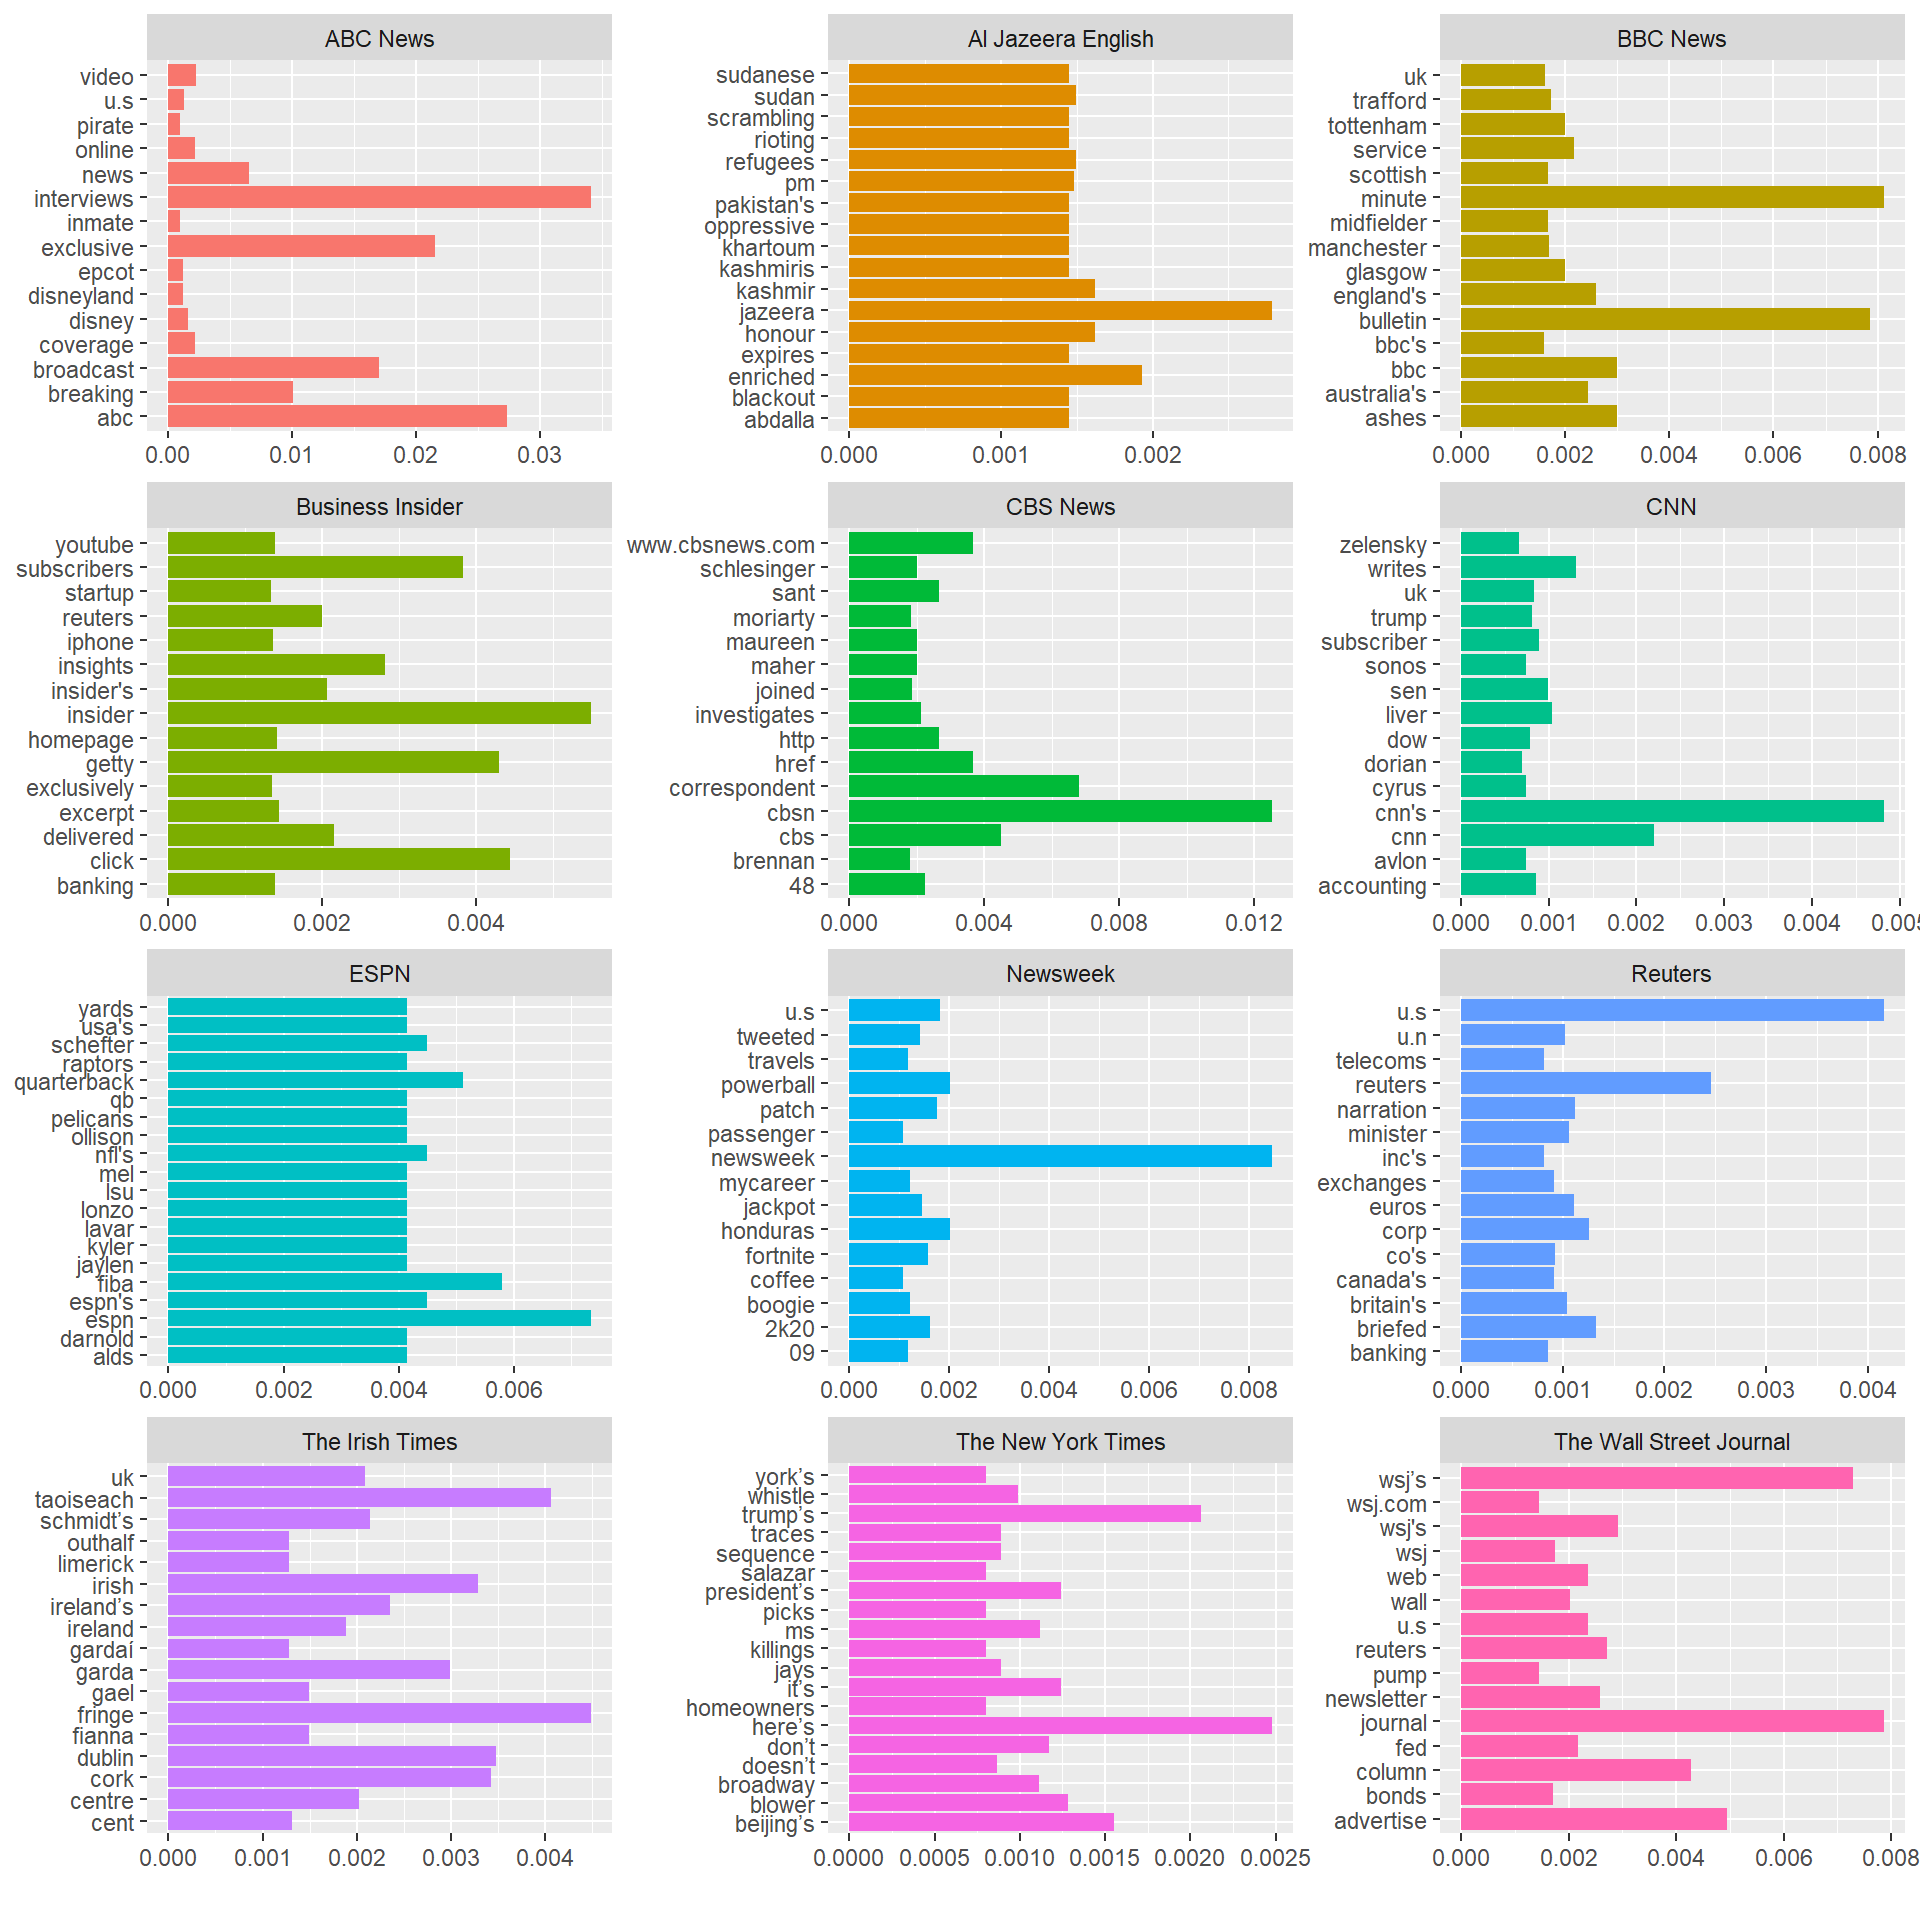
\includegraphics{index_files/figure-latex/unnamed-chunk-25-1} 

}

\caption{Figure 8 - Highest tf-idf words amongst the dataset's news sources}\label{fig:unnamed-chunk-25}
\end{figure}

Interesting to see 48 which is the 48 Hours show on CBS, the source name
and their websites is also obvious and expected. There is more football
coverage under BBC news by the words \emph{trafford} and
\emph{tottenham}, but probably needed a higher k to arrive at a sports
cluster. However, the main limitation behind this could possibly be the
diverse topics covered by ESPN such as NFL and basketball vs.~mainly
Olympics and football coverage by BBC.

\hypertarget{n-grams-and-correlation}{%
\subsubsection{N-grams and correlation}\label{n-grams-and-correlation}}

Our focus so far has been on \emph{unigrams}, however we could certainly
derive a lot more from \emph{bigrams}. Bigrams allow us to visualise the
connectivity between these words using the \texttt{igraph} package.

\begin{Shaded}
\begin{Highlighting}[]
\NormalTok{article\_bigrams }\OtherTok{\textless{}{-}}\NormalTok{ clean\_articles }\SpecialCharTok{\%\textgreater{}\%}
                    \FunctionTok{unnest\_tokens}\NormalTok{(bigrams, description, }\AttributeTok{token =} \StringTok{"ngrams"}\NormalTok{, }\AttributeTok{n =} \DecValTok{2}\NormalTok{)}
\end{Highlighting}
\end{Shaded}

Now we have unnested the \texttt{description} columns by bigrams, we can
count the frequency of unique combinations.

\begin{Shaded}
\begin{Highlighting}[]
\FunctionTok{data}\NormalTok{(stop\_words)}

\NormalTok{article\_bigrams }\OtherTok{\textless{}{-}}\NormalTok{ article\_bigrams }\SpecialCharTok{\%\textgreater{}\%}
                    \FunctionTok{count}\NormalTok{(bigrams, }\AttributeTok{sort =} \ConstantTok{TRUE}\NormalTok{)}
\end{Highlighting}
\end{Shaded}

We will now filter out any stopword occurrences after splitting the
\texttt{bigrams} into two columns for each of the two words.

\begin{Shaded}
\begin{Highlighting}[]
\NormalTok{bigrams\_split }\OtherTok{\textless{}{-}}\NormalTok{article\_bigrams }\SpecialCharTok{\%\textgreater{}\%}
  \FunctionTok{separate}\NormalTok{(bigrams, }\FunctionTok{c}\NormalTok{(}\StringTok{"word1"}\NormalTok{,}\StringTok{"word2"}\NormalTok{), }\AttributeTok{sep=} \StringTok{" "}\NormalTok{) }\SpecialCharTok{\%\textgreater{}\%}
  \FunctionTok{filter}\NormalTok{(}\SpecialCharTok{!}\NormalTok{word1 }\SpecialCharTok{\%in\%}\NormalTok{ stop\_words}\SpecialCharTok{$}\NormalTok{word) }\SpecialCharTok{\%\textgreater{}\%}
  \FunctionTok{filter}\NormalTok{(}\SpecialCharTok{!}\NormalTok{word2 }\SpecialCharTok{\%in\%}\NormalTok{ stop\_words}\SpecialCharTok{$}\NormalTok{word) }\SpecialCharTok{\%\textgreater{}\%}
  \FunctionTok{arrange}\NormalTok{(}\FunctionTok{desc}\NormalTok{(n))}
\end{Highlighting}
\end{Shaded}

Using the \texttt{igraph} package we can now visualise connectivity
between words that have occurred more than 15 times. We will also
increase the thickness of the links depending on the frequency of these
bigrams by assigning \texttt{edge\_with\ =\ n} within
\texttt{geom\_edge\_link()}. \emph{Really cool stuff!}

\begin{Shaded}
\begin{Highlighting}[]
\FunctionTok{library}\NormalTok{(ggraph)}
\FunctionTok{library}\NormalTok{(igraph)}
\FunctionTok{library}\NormalTok{(grid)}

\NormalTok{bigram\_igraph }\OtherTok{\textless{}{-}}\NormalTok{ bigrams\_split }\SpecialCharTok{\%\textgreater{}\%}
 \FunctionTok{filter}\NormalTok{(n }\SpecialCharTok{\textgreater{}} \DecValTok{15}\NormalTok{) }\SpecialCharTok{\%\textgreater{}\%}
 \FunctionTok{filter}\NormalTok{(}\SpecialCharTok{!}\FunctionTok{is.na}\NormalTok{(word1)) }\SpecialCharTok{\%\textgreater{}\%}
 \FunctionTok{filter}\NormalTok{(}\SpecialCharTok{!}\FunctionTok{is.na}\NormalTok{(word2)) }\SpecialCharTok{\%\textgreater{}\%}
 \FunctionTok{graph\_from\_data\_frame}\NormalTok{() }

\FunctionTok{set.seed}\NormalTok{(}\DecValTok{1234}\NormalTok{)}

\FunctionTok{ggraph}\NormalTok{(bigram\_igraph, }\AttributeTok{layout =} \StringTok{"fr"}\NormalTok{) }\SpecialCharTok{+} 
\FunctionTok{geom\_edge\_link}\NormalTok{(}\FunctionTok{aes}\NormalTok{(}\AttributeTok{edge\_alpha =}\NormalTok{ n, }\AttributeTok{edge\_width =}\NormalTok{ n), }\AttributeTok{edge\_colour =} \StringTok{"cyan4"}\NormalTok{, }\AttributeTok{end\_cap =} \FunctionTok{circle}\NormalTok{(}\FloatTok{0.07}\NormalTok{, }\StringTok{\textquotesingle{}inches\textquotesingle{}}\NormalTok{)) }\SpecialCharTok{+}
\FunctionTok{geom\_node\_point}\NormalTok{(}\AttributeTok{color =} \StringTok{"lightblue"}\NormalTok{, }\AttributeTok{size =} \DecValTok{5}\NormalTok{) }\SpecialCharTok{+} 
\FunctionTok{geom\_node\_text}\NormalTok{(}\FunctionTok{aes}\NormalTok{(}\AttributeTok{label =}\NormalTok{ name), }\AttributeTok{vjust =} \DecValTok{1}\NormalTok{, }\AttributeTok{hjust =} \DecValTok{1}\NormalTok{) }\SpecialCharTok{+} 
\FunctionTok{theme\_void}\NormalTok{()}
\end{Highlighting}
\end{Shaded}

\begin{figure}

{\centering 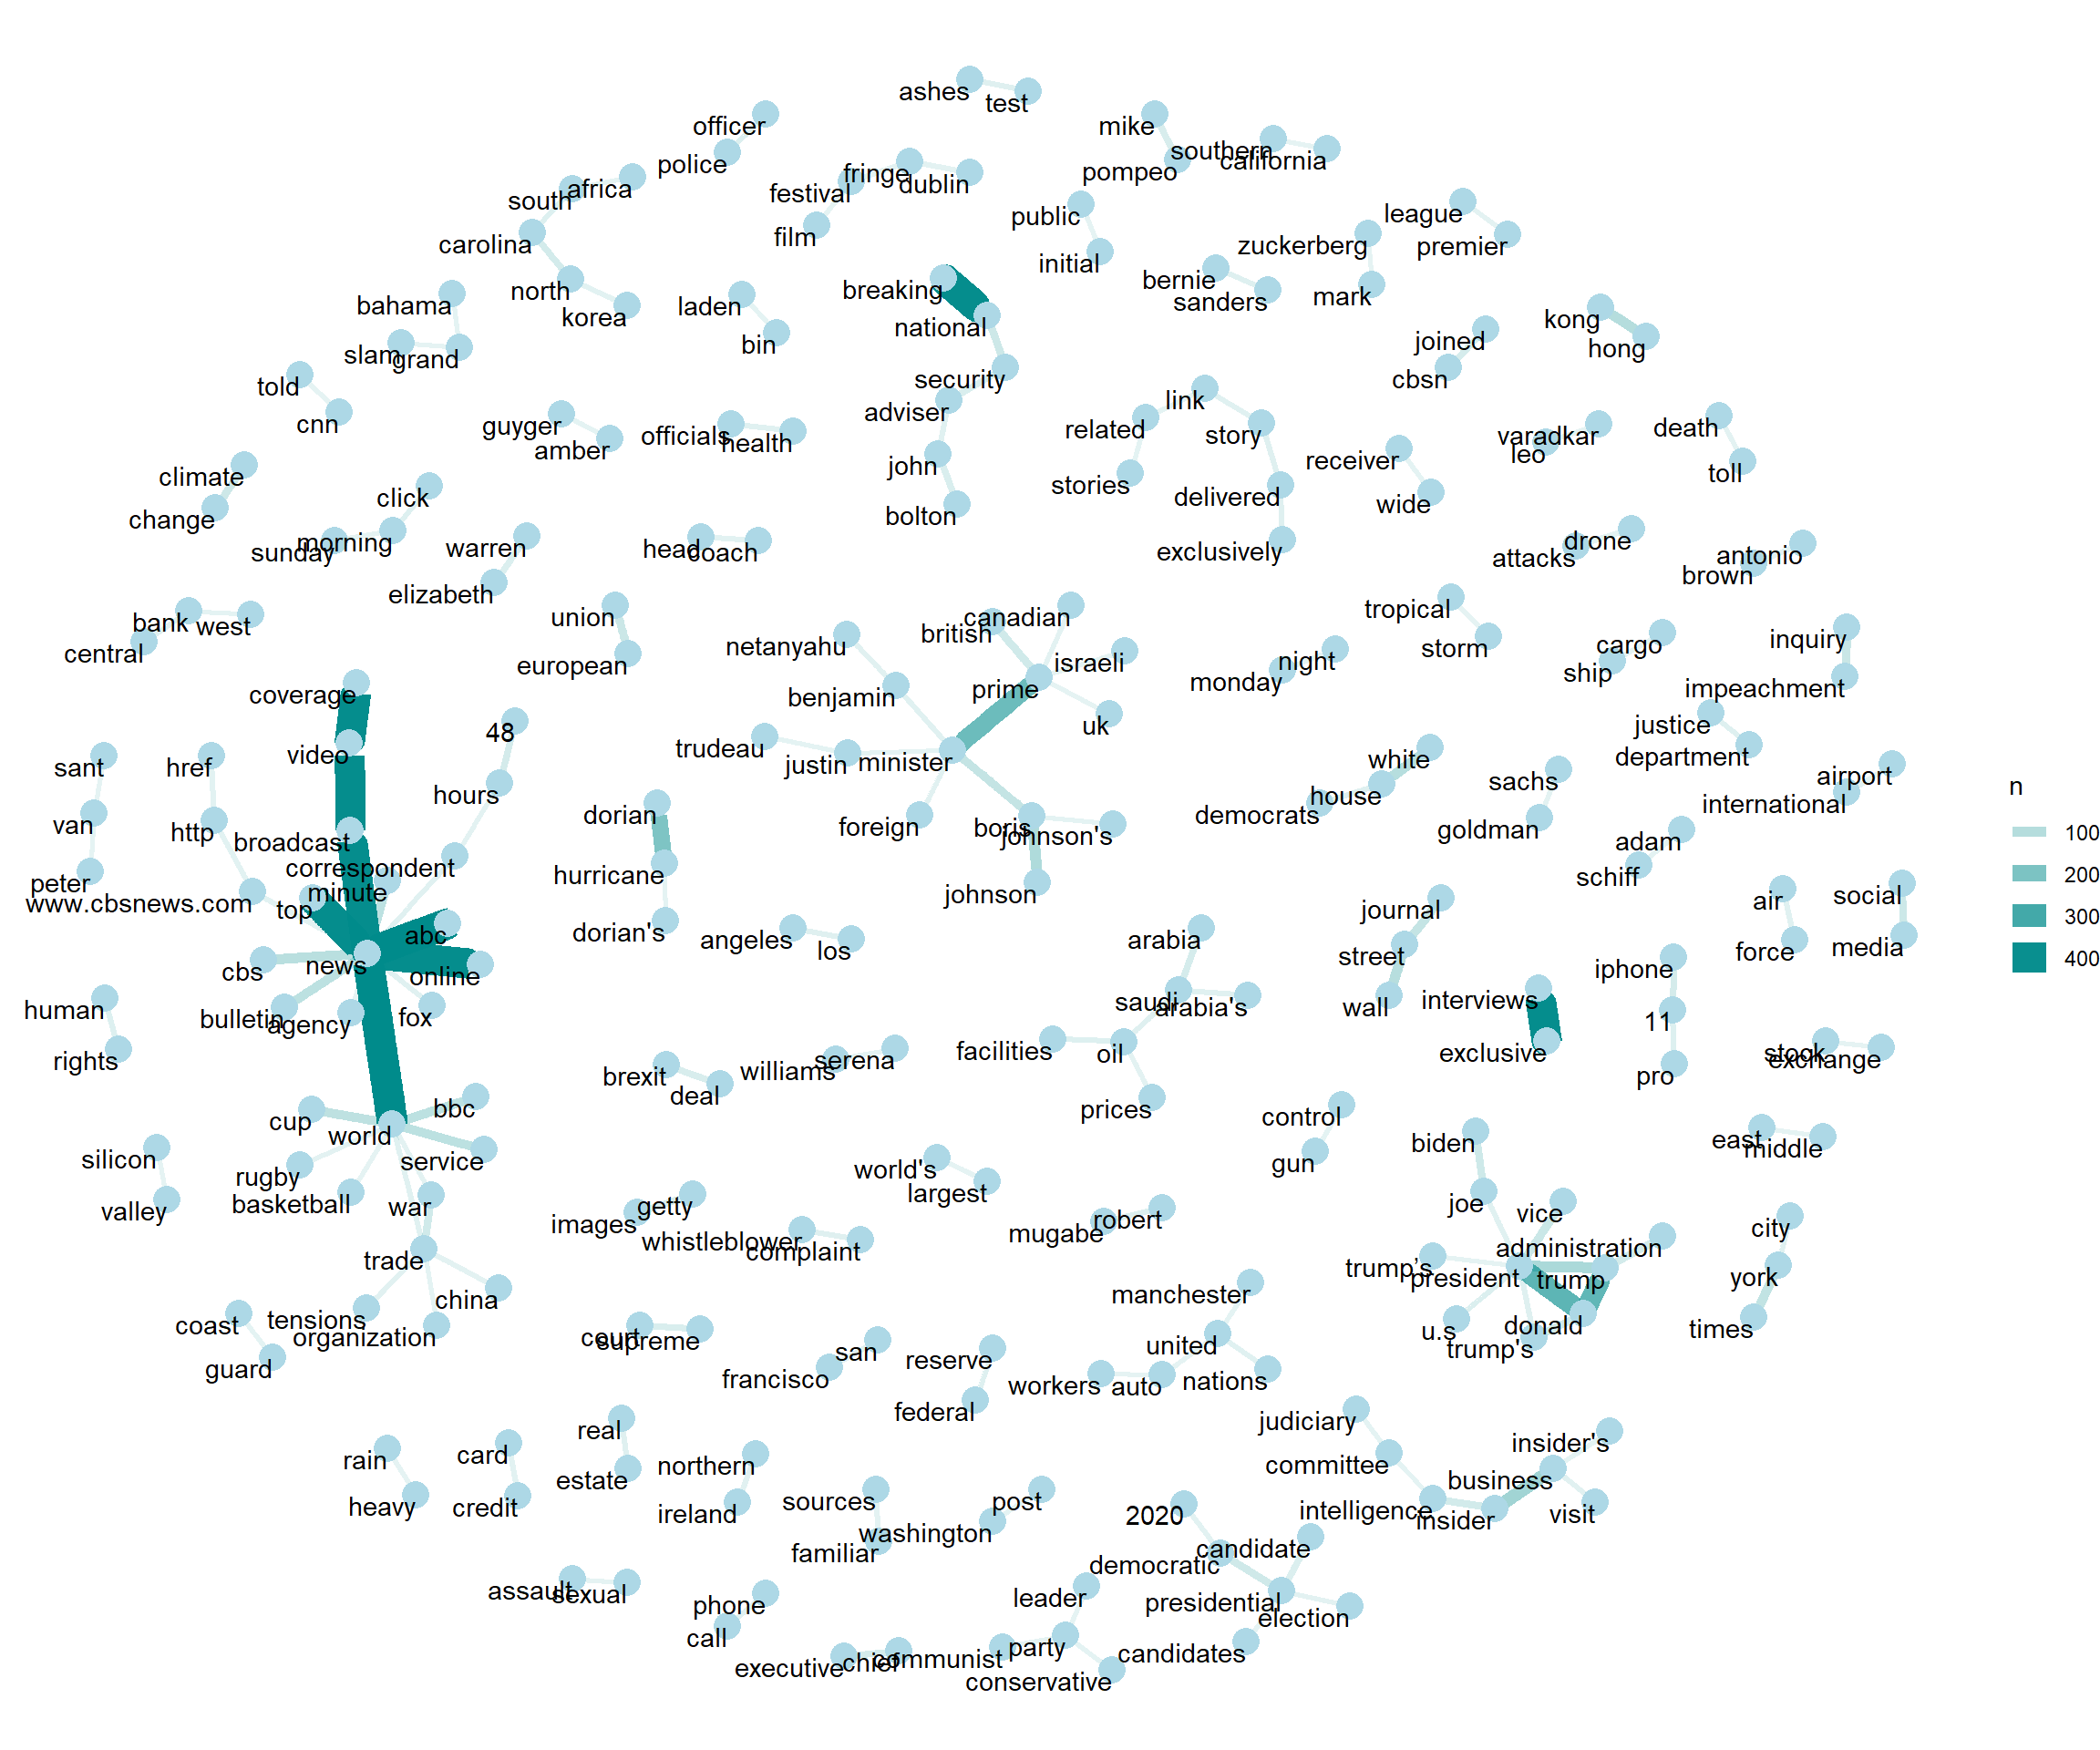
\includegraphics{index_files/figure-latex/unnamed-chunk-29-1} 

}

\caption{Figure 9 - Most recurring bigrams in all articles that have occurred at least 15 times}\label{fig:unnamed-chunk-29}
\end{figure}

We can clearly tell a story now. For example, one particular theme
surrounding US coverage was on former President Donald Trump and his
administration whilst Vice President \emph{(now President)} Joe Biden
was the runner-up.

\hypertarget{putting-the-final-pieces-together}{%
\subsubsection{Putting the final pieces
together}\label{putting-the-final-pieces-together}}

We will now combine various pieces from our final products above to form
a meaningful relationship through a linear regression model. Our aim to
explain \emph{popularity} depending on the \textbf{source name},
\textbf{sentiment}, \textbf{topic category} and \textbf{image status},
which we plan to add further below.

\hypertarget{popularity-by-source-name}{%
\paragraph{Popularity by source name}\label{popularity-by-source-name}}

We finally attempt to visualise popularity by the various sources.

\begin{Shaded}
\begin{Highlighting}[]
\NormalTok{clean\_articles }\SpecialCharTok{\%\textgreater{}\%}
\FunctionTok{mutate}\NormalTok{(}\AttributeTok{popularity =}\NormalTok{ engagement\_reaction\_count }\SpecialCharTok{+}\NormalTok{ engagement\_comment\_count }\SpecialCharTok{+}\NormalTok{ engagement\_share\_count }\SpecialCharTok{+}\NormalTok{ engagement\_comment\_plugin\_count) }\SpecialCharTok{\%\textgreater{}\%}
\FunctionTok{group\_by}\NormalTok{(source\_name) }\SpecialCharTok{\%\textgreater{}\%}
\FunctionTok{summarise}\NormalTok{(}\AttributeTok{popularity =} \FunctionTok{mean}\NormalTok{(popularity, }\AttributeTok{na.rm =}\ConstantTok{TRUE}\NormalTok{)) }\SpecialCharTok{\%\textgreater{}\%}
\FunctionTok{ggplot}\NormalTok{(}\FunctionTok{aes}\NormalTok{(}\FunctionTok{fct\_reorder}\NormalTok{(source\_name, popularity), popularity, }\AttributeTok{fill =}\NormalTok{ source\_name)) }\SpecialCharTok{+}
\FunctionTok{geom\_col}\NormalTok{(}\AttributeTok{show.legend =} \ConstantTok{FALSE}\NormalTok{) }\SpecialCharTok{+}
\FunctionTok{coord\_flip}\NormalTok{() }\SpecialCharTok{+}
\FunctionTok{ylab}\NormalTok{(}\StringTok{""}\NormalTok{) }\SpecialCharTok{+}
\FunctionTok{xlab}\NormalTok{(}\StringTok{""}\NormalTok{)}
\end{Highlighting}
\end{Shaded}

\begin{figure}

{\centering 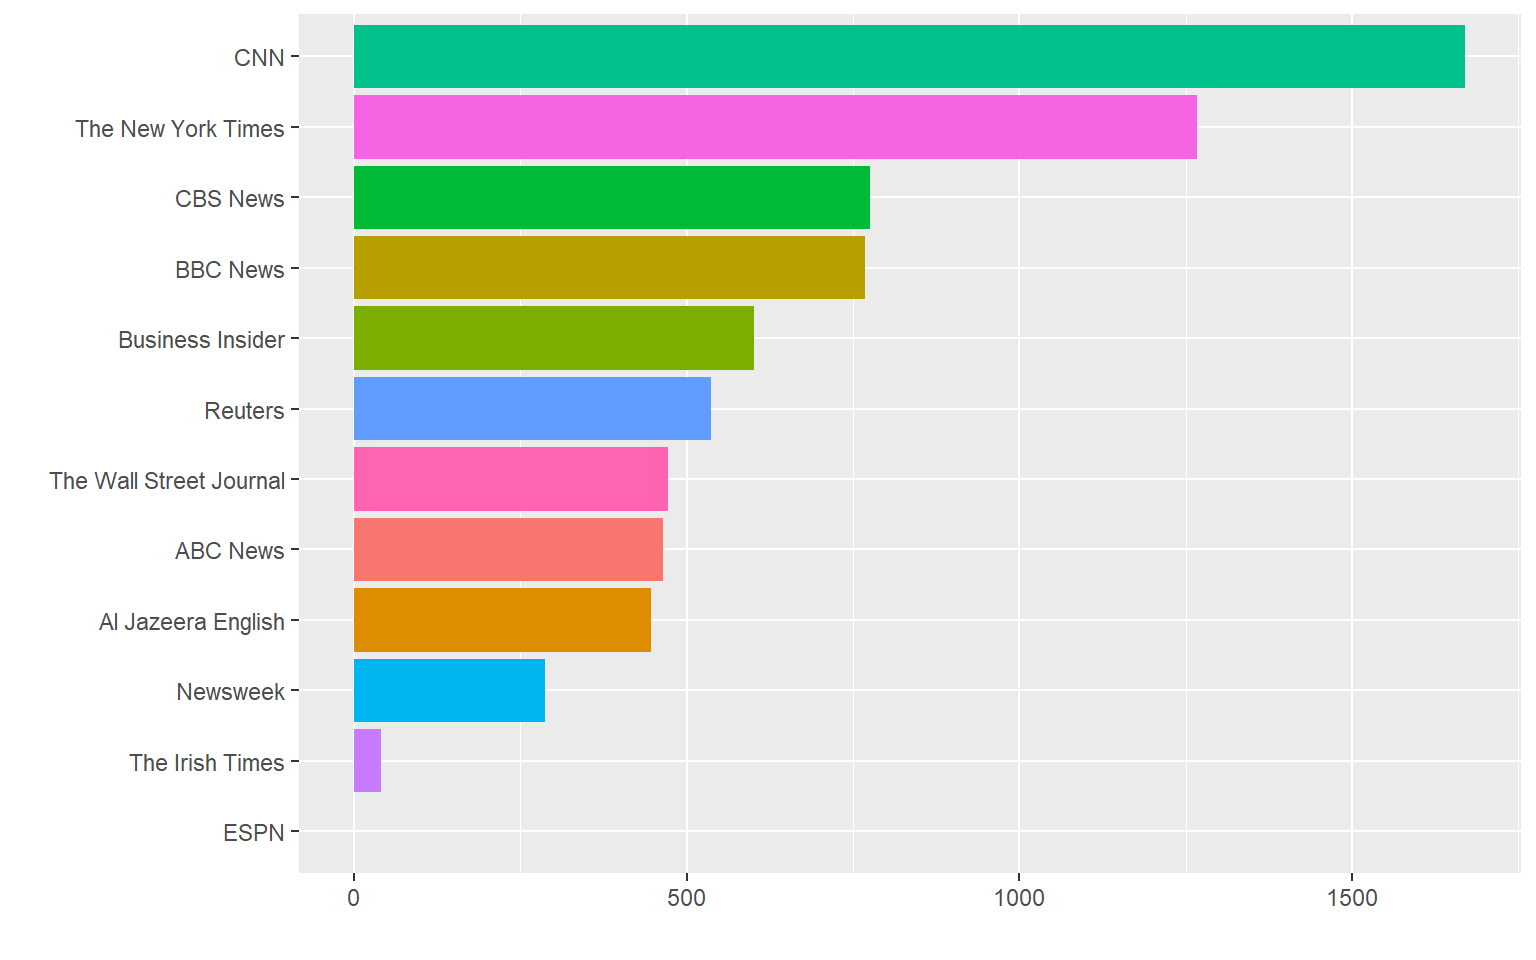
\includegraphics{index_files/figure-latex/unnamed-chunk-30-1} 

}

\caption{Figure 10 - Average popularity amongst the different news service providers}\label{fig:unnamed-chunk-30}
\end{figure}

This clearly shows that the New York Times and CNN are clear high flyers
in terms of popularity, with both the Irish Times and ESPN way below
average. This will help us regroup the middle categories as one as they
all fall within range in terms of popularity (i.e.~\emph{CBS News},
\emph{Al Jazeera English}, \emph{Newsweek}, \emph{Business Insider},
\emph{BBC News}, \emph{ABC News}, \emph{The Wall Street Journal}, and
\emph{Reuters})

\hypertarget{sentiment}{%
\subparagraph{Sentiment}\label{sentiment}}

We will also have a look at sentiment across the board

\begin{Shaded}
\begin{Highlighting}[]
\FunctionTok{library}\NormalTok{(lubridate)}

\NormalTok{clean\_articles }\SpecialCharTok{\%\textgreater{}\%}
\FunctionTok{left\_join}\NormalTok{(}
           \FunctionTok{select}\NormalTok{(sentiment\_bing, }\FunctionTok{c}\NormalTok{(}\StringTok{"article\_id"}\NormalTok{, }\StringTok{"sentiment"}\NormalTok{)}
\NormalTok{                                                              )) }\SpecialCharTok{\%\textgreater{}\%}
\FunctionTok{ggplot}\NormalTok{(}\FunctionTok{aes}\NormalTok{(sentiment, }\AttributeTok{fill =}\NormalTok{ source\_name)) }\SpecialCharTok{+}
\FunctionTok{geom\_density}\NormalTok{(}\AttributeTok{show.legend =} \ConstantTok{FALSE}\NormalTok{) }\SpecialCharTok{+} 
\FunctionTok{facet\_wrap}\NormalTok{(}\SpecialCharTok{\textasciitilde{}}\NormalTok{source\_name) }\SpecialCharTok{+}
\FunctionTok{xlab}\NormalTok{(}\StringTok{""}\NormalTok{)}
\end{Highlighting}
\end{Shaded}

\begin{figure}

{\centering 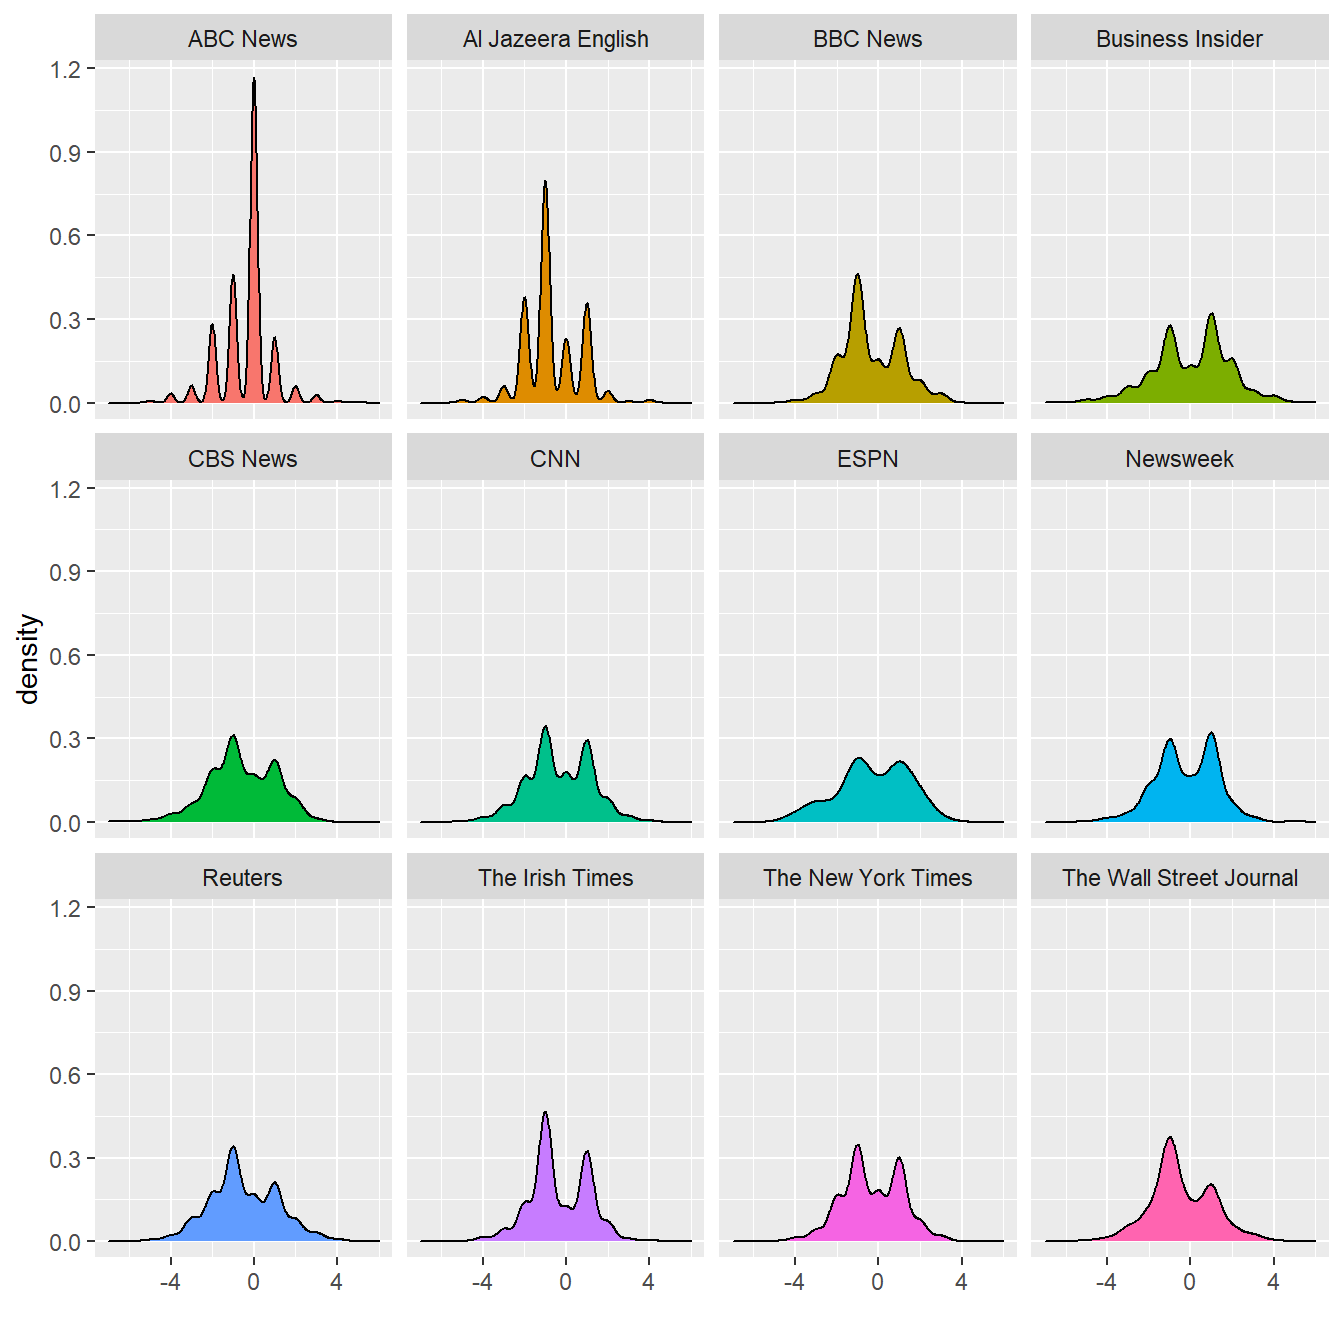
\includegraphics{index_files/figure-latex/unnamed-chunk-31-1} 

}

\caption{Figure 11 - Sentiment score distribution by News provider}\label{fig:unnamed-chunk-31}
\end{figure}

Overall sentiment looks balanced. We will take an easy shortcut by
assuming sentiment is fairly similar for now. Now, it's time for data
wrangling before we apply our lm model.

\begin{Shaded}
\begin{Highlighting}[]
\NormalTok{model\_set }\OtherTok{\textless{}{-}}\NormalTok{ clean\_articles }\SpecialCharTok{\%\textgreater{}\%}
\FunctionTok{mutate}\NormalTok{(}\AttributeTok{popularity =}\NormalTok{ engagement\_reaction\_count }\SpecialCharTok{+}\NormalTok{ engagement\_comment\_count }\SpecialCharTok{+}\NormalTok{ engagement\_share\_count }\SpecialCharTok{+}\NormalTok{ engagement\_comment\_plugin\_count) }\SpecialCharTok{\%\textgreater{}\%}
\FunctionTok{left\_join}\NormalTok{(}
           \FunctionTok{select}\NormalTok{(sentiment\_bing, }\FunctionTok{c}\NormalTok{(}\StringTok{"article\_id"}\NormalTok{, }\StringTok{"sentiment"}\NormalTok{)}
\NormalTok{                                                              )) }\SpecialCharTok{\%\textgreater{}\%}
\FunctionTok{mutate}\NormalTok{(}\AttributeTok{source\_name =} \FunctionTok{case\_when}\NormalTok{(}
\NormalTok{    source\_name }\SpecialCharTok{==} \StringTok{"CNN"}                  \SpecialCharTok{\textasciitilde{}} \StringTok{"CNN"}\NormalTok{,}
\NormalTok{    source\_name }\SpecialCharTok{==} \StringTok{"The Irish Times"}      \SpecialCharTok{\textasciitilde{}} \StringTok{"The Irish Times"}\NormalTok{,}
\NormalTok{    source\_name }\SpecialCharTok{==} \StringTok{"The New York Times"}   \SpecialCharTok{\textasciitilde{}} \StringTok{"The New York Times"}\NormalTok{,}
\NormalTok{    source\_name }\SpecialCharTok{==} \StringTok{"ESPN"}                 \SpecialCharTok{\textasciitilde{}} \StringTok{"ESPN"}\NormalTok{,}
    \ConstantTok{TRUE}                                  \SpecialCharTok{\textasciitilde{}} \StringTok{"Other"}\NormalTok{)) }\SpecialCharTok{\%\textgreater{}\%}
  \FunctionTok{mutate}\NormalTok{(}\AttributeTok{sentiment\_cat =} \FunctionTok{case\_when}\NormalTok{(}
\NormalTok{    sentiment }\SpecialCharTok{\textgreater{}} \DecValTok{0}                  \SpecialCharTok{\textasciitilde{}} \StringTok{"positive"}\NormalTok{,}
\NormalTok{    sentiment }\SpecialCharTok{\textless{}} \DecValTok{0}                  \SpecialCharTok{\textasciitilde{}} \StringTok{"negative"}\NormalTok{,}
    \ConstantTok{TRUE}                           \SpecialCharTok{\textasciitilde{}} \StringTok{"neutral"}\NormalTok{)) }\SpecialCharTok{\%\textgreater{}\%}
\FunctionTok{mutate}\NormalTok{(}\AttributeTok{image\_status =} \FunctionTok{if\_else}\NormalTok{(}\FunctionTok{is.na}\NormalTok{(url\_to\_image), }\DecValTok{0}\NormalTok{, }\DecValTok{1}\NormalTok{)) }\SpecialCharTok{\%\textgreater{}\%}
\FunctionTok{left\_join}\NormalTok{(articles\_gamma\_sliced)}

\NormalTok{model\_lm }\OtherTok{\textless{}{-}} \FunctionTok{lm}\NormalTok{(}\AttributeTok{formula =}\NormalTok{ popularity }\SpecialCharTok{\textasciitilde{}}\NormalTok{ sentiment\_cat }\SpecialCharTok{+}\NormalTok{ topic\_category }\SpecialCharTok{+}\NormalTok{ source\_name }\SpecialCharTok{+}\NormalTok{ image\_status, }\AttributeTok{data =}\NormalTok{ model\_set)}
        
\FunctionTok{summary}\NormalTok{(model\_lm)}
\end{Highlighting}
\end{Shaded}

\begin{verbatim}
## 
## Call:
## lm(formula = popularity ~ sentiment_cat + topic_category + source_name + 
##     image_status, data = model_set)
## 
## Residuals:
##    Min     1Q Median     3Q    Max 
##  -2211   -742   -475    -72 432644 
## 
## Coefficients:
##                                      Estimate Std. Error
## (Intercept)                           1074.09     346.25
## sentiment_catneutral                    40.51     138.39
## sentiment_catpositive                 -165.15     161.50
## topic_categoryEconomy and Trade       -138.35     202.16
## topic_categoryExclusive content       -322.35     238.58
## topic_categoryInternational coverage   100.59     203.45
## topic_categoryUK coverage              -89.16     210.20
## topic_categoryUS coverage              600.01     208.24
## source_nameESPN                      -1494.24     692.71
## source_nameOther                      -957.37     195.31
## source_nameThe Irish Times           -1505.12     257.40
## source_nameThe New York Times         -380.09     262.83
## image_status                           496.51     254.12
##                                      t value Pr(>|t|)
## (Intercept)                            3.102  0.00193
## sentiment_catneutral                   0.293  0.76974
## sentiment_catpositive                 -1.023  0.30653
## topic_categoryEconomy and Trade       -0.684  0.49376
## topic_categoryExclusive content       -1.351  0.17669
## topic_categoryInternational coverage   0.494  0.62100
## topic_categoryUK coverage             -0.424  0.67145
## topic_categoryUS coverage              2.881  0.00397
## source_nameESPN                       -2.157  0.03102
## source_nameOther                      -4.902 9.65e-07
## source_nameThe Irish Times            -5.847 5.14e-09
## source_nameThe New York Times         -1.446  0.14817
## image_status                           1.954  0.05074
##                                         
## (Intercept)                          ** 
## sentiment_catneutral                    
## sentiment_catpositive                   
## topic_categoryEconomy and Trade         
## topic_categoryExclusive content         
## topic_categoryInternational coverage    
## topic_categoryUK coverage               
## topic_categoryUS coverage            ** 
## source_nameESPN                      *  
## source_nameOther                     ***
## source_nameThe Irish Times           ***
## source_nameThe New York Times           
## image_status                         .  
## ---
## Signif. codes:  
## 0 '***' 0.001 '**' 0.01 '*' 0.05 '.' 0.1 ' ' 1
## 
## Residual standard error: 6027 on 10306 degrees of freedom
##   (117 observations deleted due to missingness)
## Multiple R-squared:  0.008083,   Adjusted R-squared:  0.006928 
## F-statistic: 6.999 on 12 and 10306 DF,  p-value: 8.14e-13
\end{verbatim}

The New York Times didn't turn to very significant, so we will regroup
with other. We will also categorise content as being either US coverage
or other

\begin{Shaded}
\begin{Highlighting}[]
\NormalTok{final\_model\_set }\OtherTok{\textless{}{-}}\NormalTok{ clean\_articles }\SpecialCharTok{\%\textgreater{}\%}
\FunctionTok{mutate}\NormalTok{(}\AttributeTok{popularity =}\NormalTok{ engagement\_reaction\_count }\SpecialCharTok{+}\NormalTok{ engagement\_comment\_count }\SpecialCharTok{+}\NormalTok{ engagement\_share\_count }\SpecialCharTok{+}\NormalTok{ engagement\_comment\_plugin\_count) }\SpecialCharTok{\%\textgreater{}\%}
\FunctionTok{left\_join}\NormalTok{(}
           \FunctionTok{select}\NormalTok{(sentiment\_bing, }\FunctionTok{c}\NormalTok{(}\StringTok{"article\_id"}\NormalTok{, }\StringTok{"sentiment"}\NormalTok{)}
\NormalTok{                                                              )) }\SpecialCharTok{\%\textgreater{}\%}
\FunctionTok{mutate}\NormalTok{(}\AttributeTok{source\_name =} \FunctionTok{case\_when}\NormalTok{(}
\NormalTok{    source\_name }\SpecialCharTok{==} \StringTok{"CNN"}                  \SpecialCharTok{\textasciitilde{}} \StringTok{"CNN"}\NormalTok{,}
\NormalTok{    source\_name }\SpecialCharTok{==} \StringTok{"The Irish Times"}      \SpecialCharTok{\textasciitilde{}} \StringTok{"The Irish Times"}\NormalTok{,}
\NormalTok{    source\_name }\SpecialCharTok{==} \StringTok{"ESPN"}                 \SpecialCharTok{\textasciitilde{}} \StringTok{"ESPN"}\NormalTok{,}
    \ConstantTok{TRUE}                                  \SpecialCharTok{\textasciitilde{}} \StringTok{"Other"}\NormalTok{)) }\SpecialCharTok{\%\textgreater{}\%}
\FunctionTok{mutate}\NormalTok{(}\AttributeTok{image\_status =} \FunctionTok{if\_else}\NormalTok{(}\FunctionTok{is.na}\NormalTok{(url\_to\_image), }\DecValTok{0}\NormalTok{, }\DecValTok{1}\NormalTok{)) }\SpecialCharTok{\%\textgreater{}\%}
\FunctionTok{left\_join}\NormalTok{(articles\_gamma\_sliced)  }\SpecialCharTok{\%\textgreater{}\%}
 \FunctionTok{mutate}\NormalTok{(}\AttributeTok{topic\_category =} \FunctionTok{case\_when}\NormalTok{(}
\NormalTok{    topic\_category }\SpecialCharTok{==} \StringTok{"US coverage"}   \SpecialCharTok{\textasciitilde{}} \StringTok{"US coverage"}\NormalTok{,}
    \ConstantTok{TRUE}                               \SpecialCharTok{\textasciitilde{}} \StringTok{"Other coverage"}\NormalTok{))}

\NormalTok{final\_model\_lm }\OtherTok{\textless{}{-}} \FunctionTok{lm}\NormalTok{(}\AttributeTok{formula =}\NormalTok{ popularity }\SpecialCharTok{\textasciitilde{}} \SpecialCharTok{+} \FunctionTok{factor}\NormalTok{(topic\_category) }\SpecialCharTok{+}\NormalTok{ source\_name }\SpecialCharTok{+}\NormalTok{ image\_status, }\AttributeTok{data =}\NormalTok{ final\_model\_set)}
        
\FunctionTok{summary}\NormalTok{(final\_model\_lm)}
\end{Highlighting}
\end{Shaded}

\begin{verbatim}
## 
## Call:
## lm(formula = popularity ~ +factor(topic_category) + source_name + 
##     image_status, data = final_model_set)
## 
## Residuals:
##    Min     1Q Median     3Q    Max 
##  -2167   -593   -577     -8 432688 
## 
## Coefficients:
##                                   Estimate Std. Error
## (Intercept)                          895.9      303.7
## factor(topic_category)US coverage    688.8      158.0
## source_nameESPN                    -1553.9      690.0
## source_nameOther                    -884.8      193.0
## source_nameThe Irish Times         -1498.3      256.1
## image_status                         582.4      245.5
##                                   t value Pr(>|t|)    
## (Intercept)                         2.951  0.00318 ** 
## factor(topic_category)US coverage   4.361 1.31e-05 ***
## source_nameESPN                    -2.252  0.02435 *  
## source_nameOther                   -4.584 4.62e-06 ***
## source_nameThe Irish Times         -5.850 5.06e-09 ***
## image_status                        2.373  0.01768 *  
## ---
## Signif. codes:  
## 0 '***' 0.001 '**' 0.01 '*' 0.05 '.' 0.1 ' ' 1
## 
## Residual standard error: 6029 on 10313 degrees of freedom
##   (117 observations deleted due to missingness)
## Multiple R-squared:  0.006721,   Adjusted R-squared:  0.00624 
## F-statistic: 13.96 on 5 and 10313 DF,  p-value: 1.265e-13
\end{verbatim}

Finally, we can formulate our statistically significant formula as
follows:

\textbf{Popularity = 895.9 + 688.8 US\_Coverage - 884.8
Other\_than\_CNN\_Source - 1498.3 The\_Irish\_Times\_Source - 1553.9
ESPN\_Source + 582.4 With\_Image}

\textbf{Interesting indeed, with all results now significant!} We can
now fairly conclude that US topics, on average are more popular than any
other topic category. Thanks to our unsupervised classification and the
amazing tidytext and stm packages.

CNN is also largely superior in terms of popularity, and is on average
above its peers by c.~885 reactions/comments/shares.

ESPN and the Irish Times aren't so popular on facebook. Probably users
rely mostly on other platforms such as Twitter or Instagram, which makes
a lot sense for ESPN users given the most likely younger generation of
followers

\emph{What's good to know is that having an image boosts popularity by
582, so definitely worth adding an image before you publish your
article!}

\end{document}
